\secnumberlesssection{ANEXOS}

\section{Matrices de contingencia del agrupamiento K-Means}
\label{anexo:matrices_kmeans}

Se presentan las tablas de contingencia que detallan la distribución cuantitativa de cada clúster descubierto por el algoritmo \textit{K-Means} ($k=4$). 
\begin{table}[H]
\centering
\caption{Tabla de contingencia: Distribución de planos anatómicos por clúster para el dominio de características cinemáticas.}
\label{tab:anexo_cinematico}
\resizebox{\textwidth}{!}{
\begin{tabular}{lcccccccc}
\hline
 & \multicolumn{2}{c}{\textbf{Fantoma Normal}} & \multicolumn{2}{c}{\textbf{Estenosis 9 mm}} & \multicolumn{2}{c}{\textbf{Estenosis 11 mm}} & \multicolumn{2}{c}{\textbf{Estenosis 13 mm}} \\ \cline{2-9} 
\textbf{Clúster asignado} & \textit{Rest} & \textit{Stress} & \textit{Rest} & \textit{Stress} & \textit{Rest} & \textit{Stress} & \textit{Rest} & \textit{Stress} \\ \hline
\textbf{Clúster 1} & 12 & 16 & 19 & 16 & 28 & 29 & 30 & 36 \\
\textbf{Clúster 2} & 0 & 0 & 20 & 26 & 8 & 11 & 0 & 0 \\
\textbf{Clúster 3} & 67 & 63 & 39 & 34 & 42 & 36 & 48 & 40 \\
\textbf{Clúster 4} & 11 & 11 & 12 & 14 & 12 & 14 & 12 & 14 \\ \hline
\end{tabular}
}
\end{table}

\begin{table}[H]
\centering
\caption{Tabla de contingencia: Distribución de planos anatómicos por clúster para el dominio de características acústicas.}
\label{tab:anexo_acustico}
\resizebox{\textwidth}{!}{
\begin{tabular}{lcccccccc}
\hline
 & \multicolumn{2}{c}{\textbf{Fantoma Normal}} & \multicolumn{2}{c}{\textbf{Estenosis 9 mm}} & \multicolumn{2}{c}{\textbf{Estenosis 11 mm}} & \multicolumn{2}{c}{\textbf{Estenosis 13 mm}} \\ \cline{2-9} 
\textbf{Clúster asignado} & \textit{Rest} & \textit{Stress} & \textit{Rest} & \textit{Stress} & \textit{Rest} & \textit{Stress} & \textit{Rest} & \textit{Stress} \\ \hline
\textbf{Clúster 1} & 48 & 22 & 24 & 10 & 28 & 11 & 30 & 12 \\
\textbf{Clúster 2} & 4 & 7 & 17 & 24 & 10 & 14 & 8 & 15 \\
\textbf{Clúster 3} & 0 & 45 & 9 & 47 & 4 & 58 & 3 & 52 \\
\textbf{Clúster 4} & 38 & 16 & 40 & 9 & 48 & 7 & 49 & 11 \\ \hline
\end{tabular}
}
\end{table}

\begin{table}[H]
\centering
\caption{Tabla de contingencia: Distribución de planos anatómicos por clúster para el dominio multimodal.}
\label{tab:anexo_multimodal}
\resizebox{\textwidth}{!}{
\begin{tabular}{lcccccccc}
\hline
 & \multicolumn{2}{c}{\textbf{Fantoma Normal}} & \multicolumn{2}{c}{\textbf{Estenosis 9 mm}} & \multicolumn{2}{c}{\textbf{Estenosis 11 mm}} & \multicolumn{2}{c}{\textbf{Estenosis 13 mm}} \\ \cline{2-9} 
\textbf{Clúster asignado} & \textit{Rest} & \textit{Stress} & \textit{Rest} & \textit{Stress} & \textit{Rest} & \textit{Stress} & \textit{Rest} & \textit{Stress} \\ \hline
\textbf{Clúster 1} & 14 & 49 & 29 & 30 & 31 & 37 & 31 & 47 \\
\textbf{Clúster 2} & 3 & 6 & 23 & 36 & 16 & 28 & 7 & 16 \\
\textbf{Clúster 3} & 11 & 11 & 12 & 13 & 13 & 13 & 14 & 14 \\
\textbf{Clúster 4} & 62 & 24 & 26 & 11 & 30 & 12 & 38 & 13 \\ \hline
\end{tabular}
}
\end{table}

\section{Exploración perceptiva y espectral bajo condición de reposo (\textit{rest})}
\label{anexo:comparacion_casos}
En este anexo se documenta la evolución espectral y acústica de los cuatro modelos morfológicos (Normal, 13 mm, 11 mm y 9 mm) evaluados bajo la condición hemodinámica de reposo (\textit{rest}). Se mantiene la misma discretización espacial definida en el análisis principal para facilitar la comparación cruzada.

\subsection{Análisis comparativo: Aorta ascendente (plano 21)}

\begin{figure}[H]
    \centering
    \begin{minipage}{0.75\textwidth}
        \begin{subfigure}{0.48\linewidth}
            \centering
            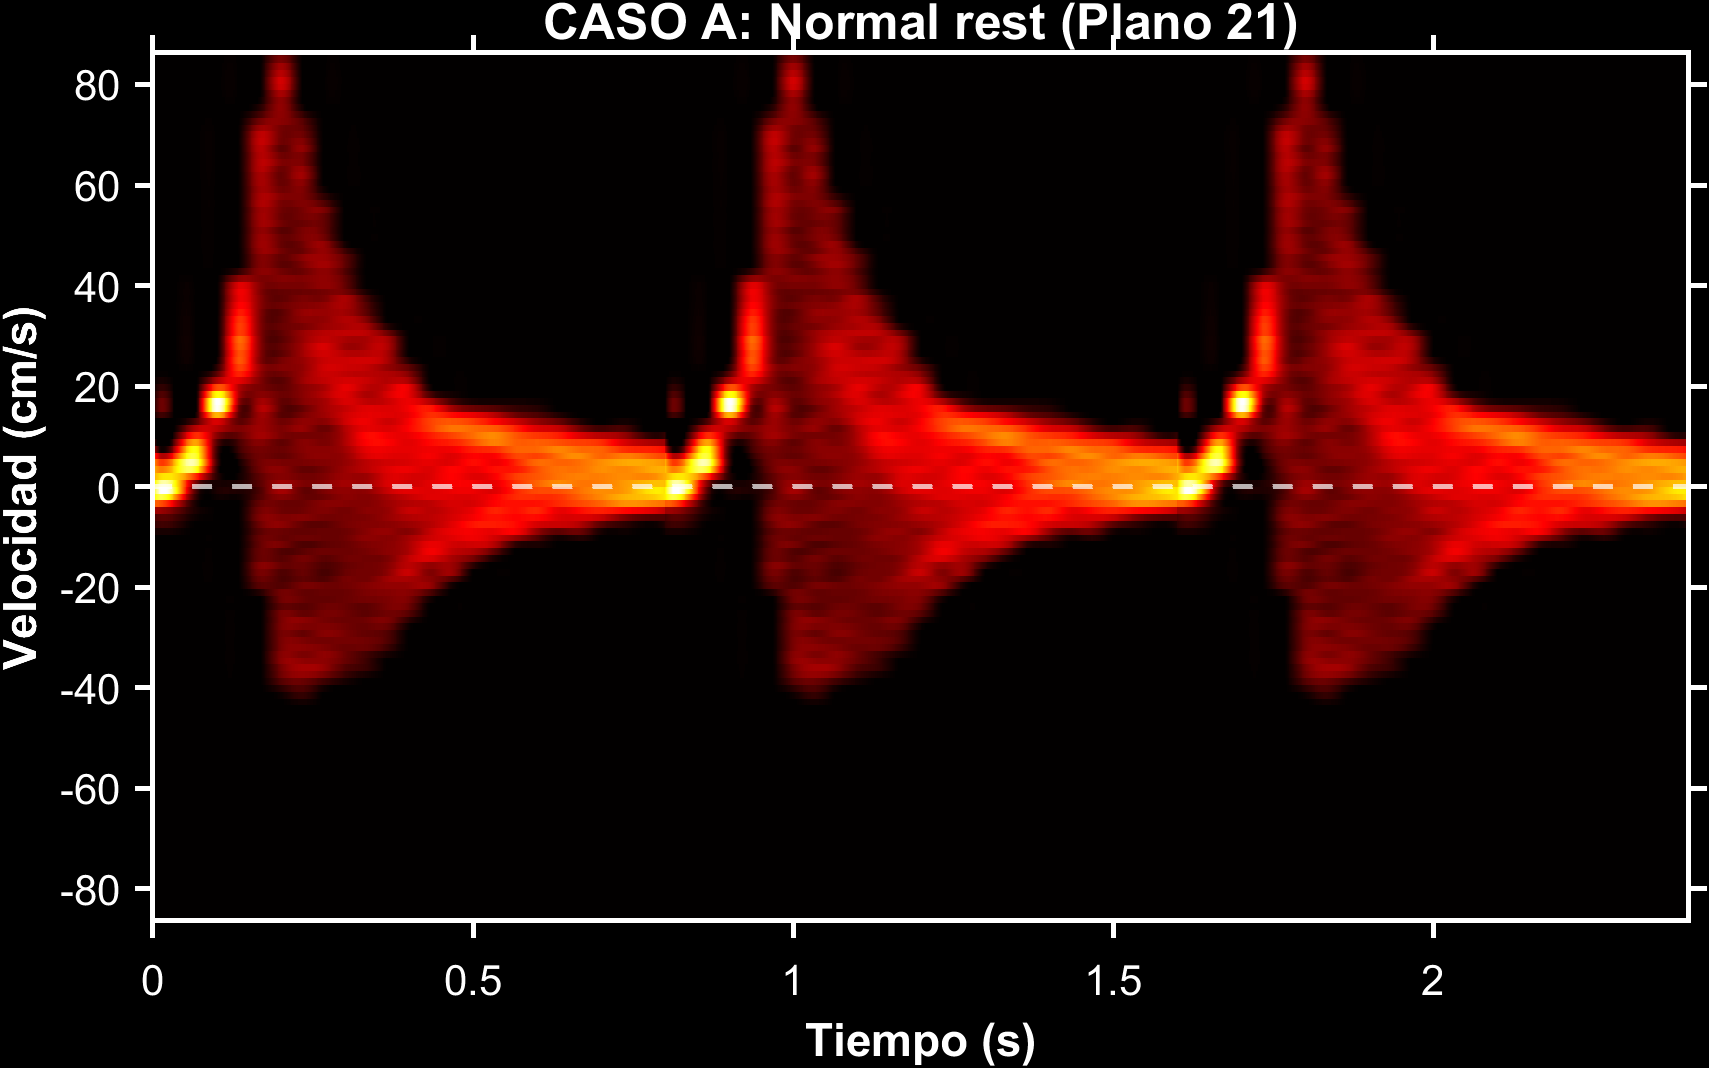
\includegraphics[width=\linewidth]{figures/anexos/Normal_rest_Plano21.png}
            \caption{\href{https://drive.google.com/file/d/1ZKAqWONgGDq1fNld8xxtLIQJTtJ9YBZD/view?usp=sharing}{Fantoma normal \textbf{(Escuchar)}}}
            \label{fig:anexo_p21_normal}
        \end{subfigure}\hfill
        \begin{subfigure}{0.48\linewidth}
            \centering
            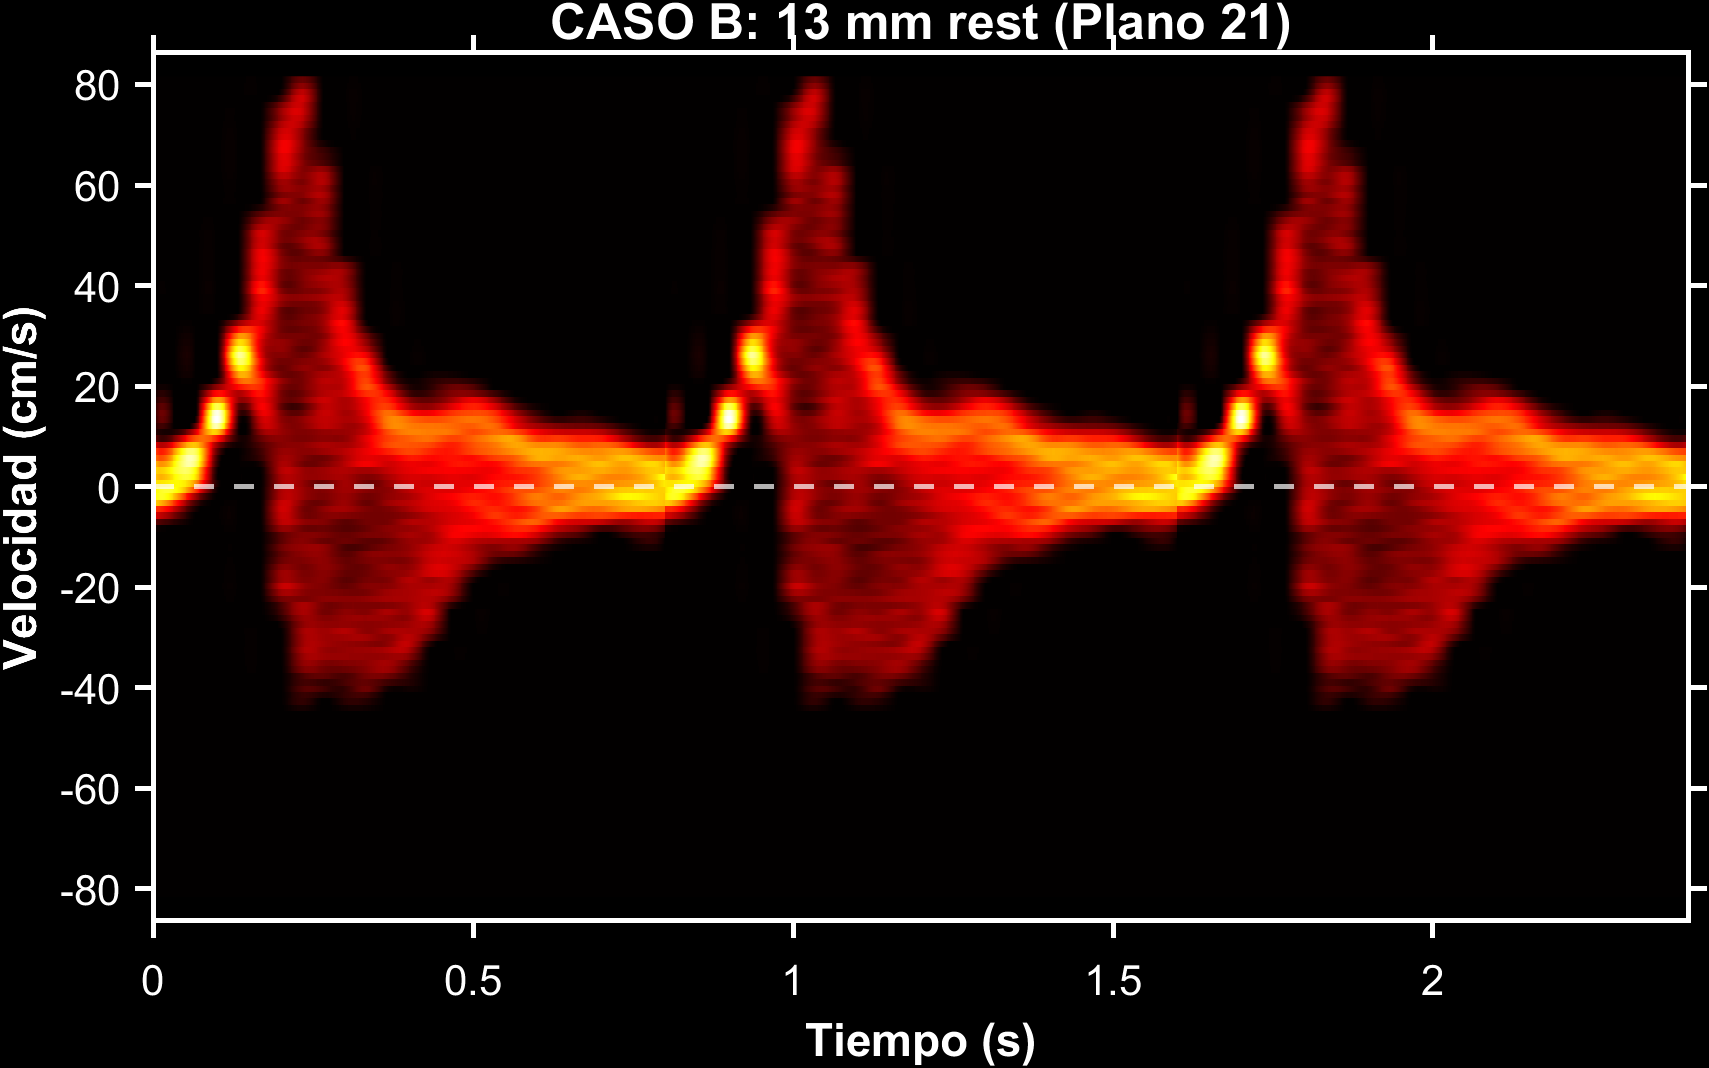
\includegraphics[width=\linewidth]{figures/anexos/13_mm_rest_Plano21.png}
            \caption{\href{https://drive.google.com/file/d/1NNRotryh_QmV-Zc-VIlffoJ7tDrSEmsP/view?usp=sharing}{Fantoma 13 mm \textbf{(Escuchar)}}}
            \label{fig:anexo_p21_13mm}
        \end{subfigure}
        
        \vspace{0.4cm}
        
        \begin{subfigure}{0.48\linewidth}
            \centering
            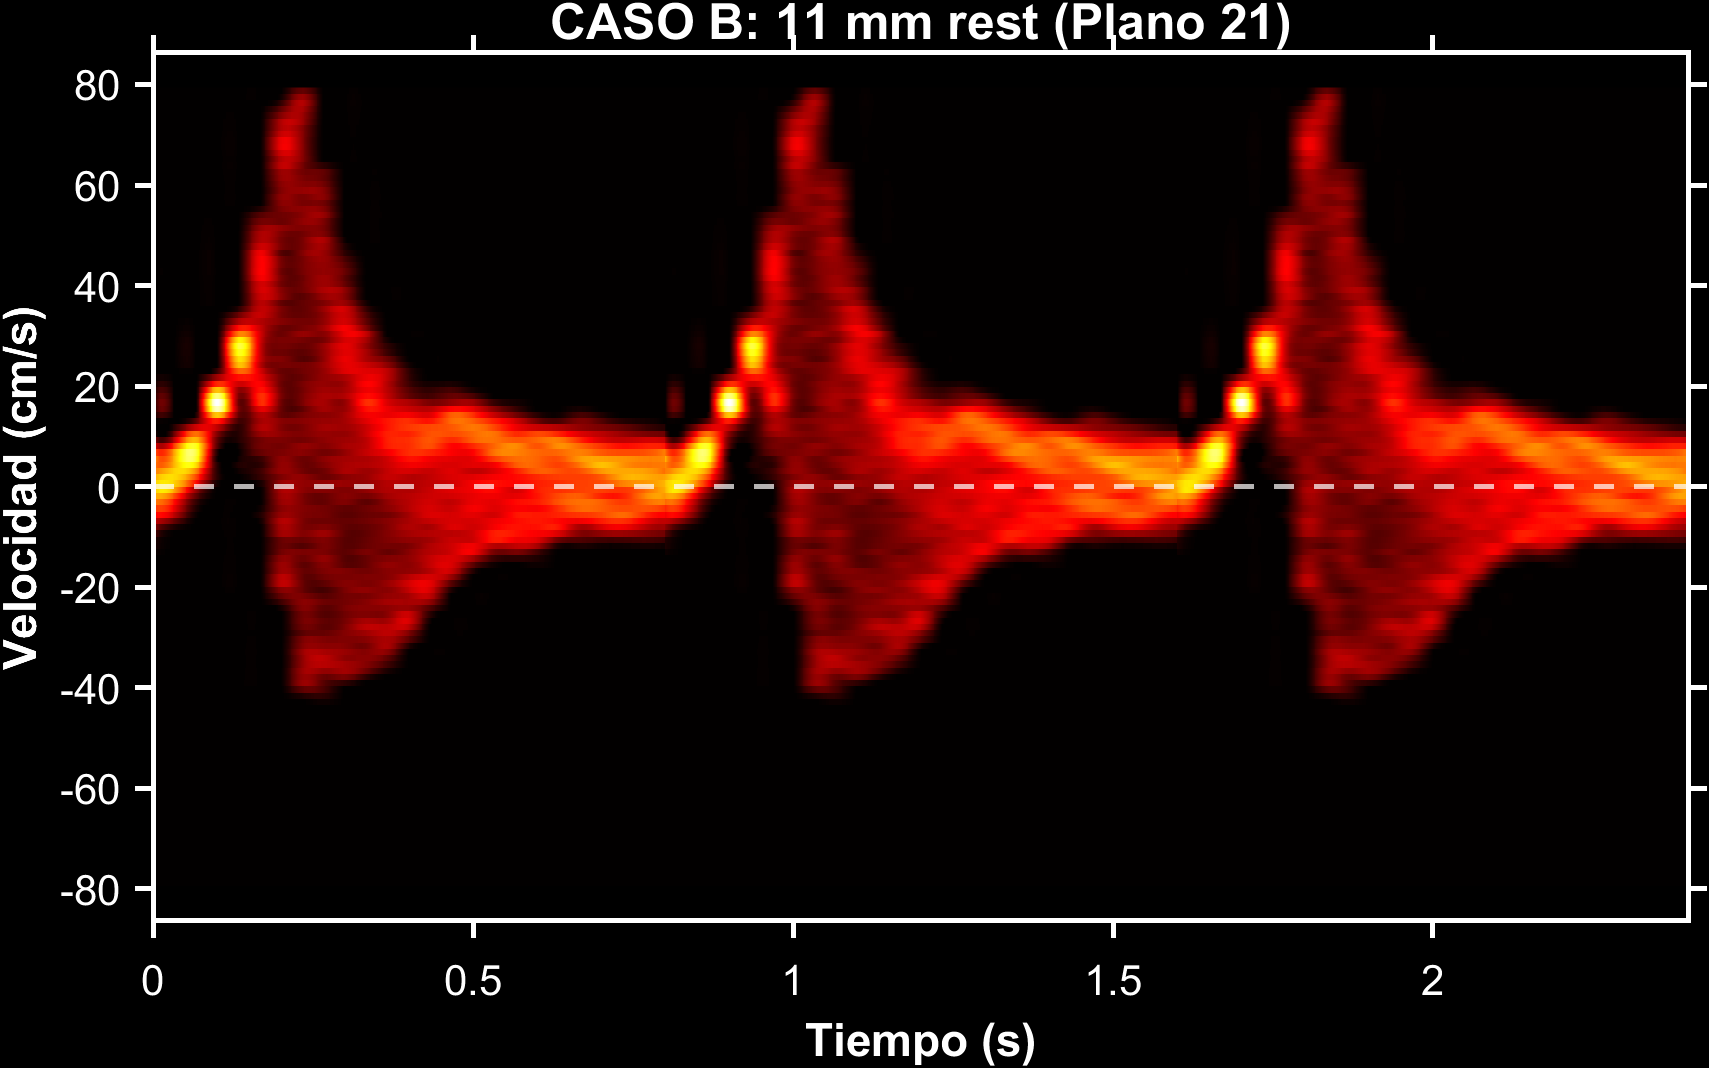
\includegraphics[width=\linewidth]{figures/anexos/11_mm_rest_Plano21.png}
            \caption{\href{https://drive.google.com/file/d/1eQq_XtXl69I2DC_eBFoO1hlGUNPU-k-t/view?usp=sharing}{Fantoma 11 mm \textbf{(Escuchar)}}}
            \label{fig:anexo_p21_11mm}
        \end{subfigure}\hfill
        \begin{subfigure}{0.48\linewidth}
            \centering
            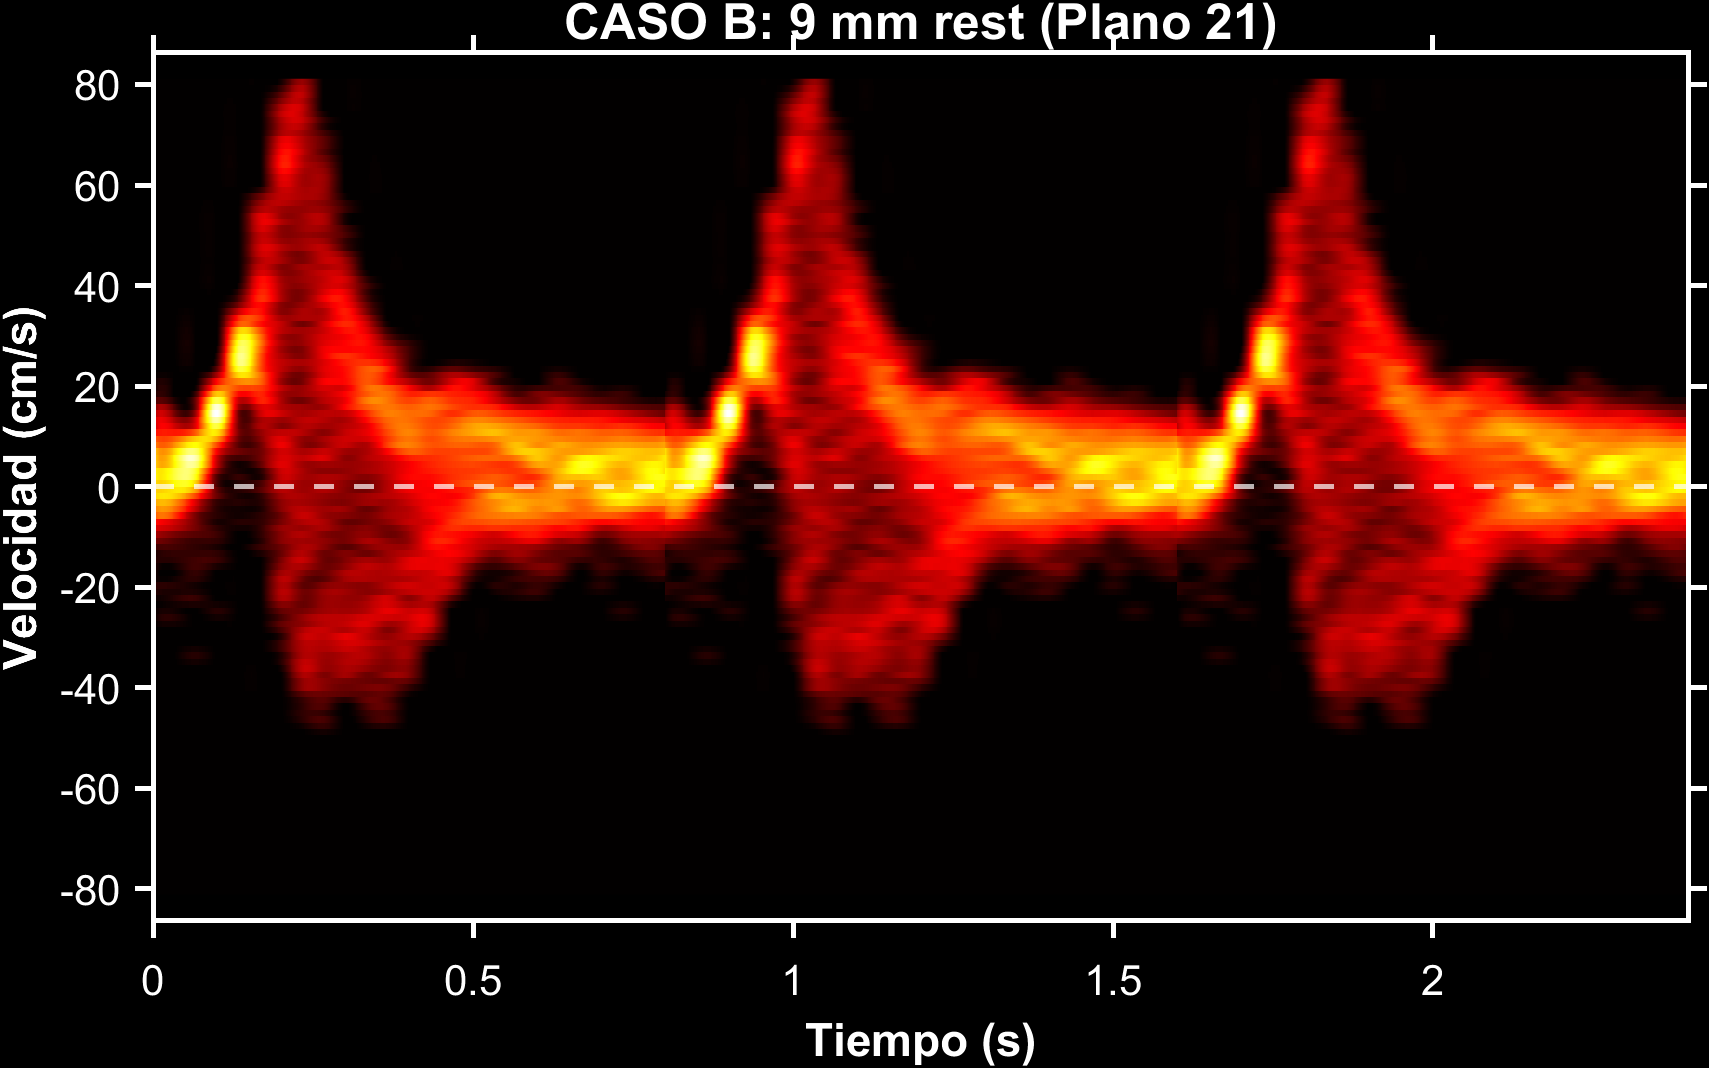
\includegraphics[width=\linewidth]{figures/anexos/9_mm_rest_Plano21.png}
            \caption{\href{https://drive.google.com/file/d/1aXkjKpO1hv90QrdGfdTchuTl22igPRqt/view?usp=sharing}{Fantoma 9 mm \textbf{(Escuchar)}}}
            \label{fig:anexo_p21_9mm}
        \end{subfigure}
    \end{minipage}
    \caption{\label{fig:anexo_comparacion_p21} Evolución espectral en la zona de la aorta ascendente bajo condición de reposo. Fuente: Elaboración propia.}
\end{figure}


\subsection{Análisis comparativo: Arco aórtico (plano 45)}

\begin{figure}[H]
    \centering
    \begin{minipage}{0.75\textwidth}
        \begin{subfigure}{0.48\linewidth}
            \centering
            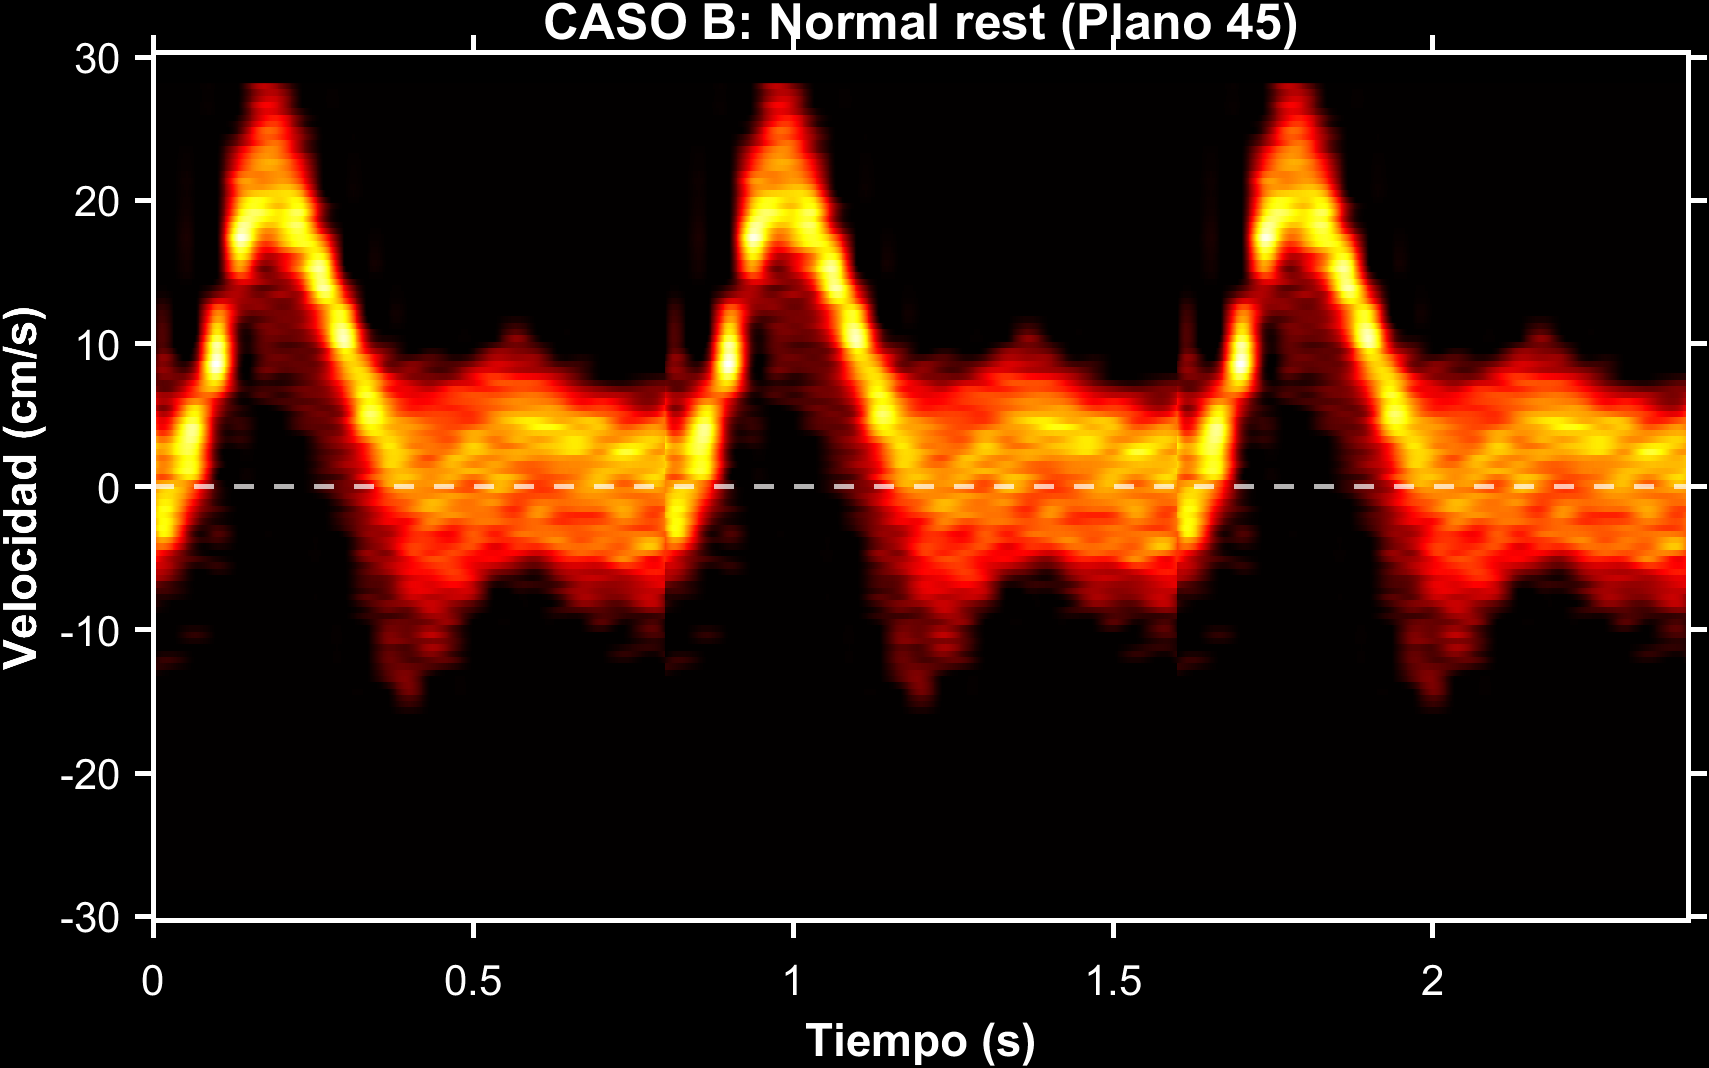
\includegraphics[width=\linewidth]{figures/anexos/Normal_rest_Plano45.png}
            \caption{\href{https://drive.google.com/file/d/1bsp7yoFzJn6wdYWwkefdBuo5repDJPdR/view?usp=sharing}{Fantoma normal \textbf{(Escuchar)}}}
            \label{fig:anexo_p45_normal}
        \end{subfigure}\hfill
        \begin{subfigure}{0.48\linewidth}
            \centering
            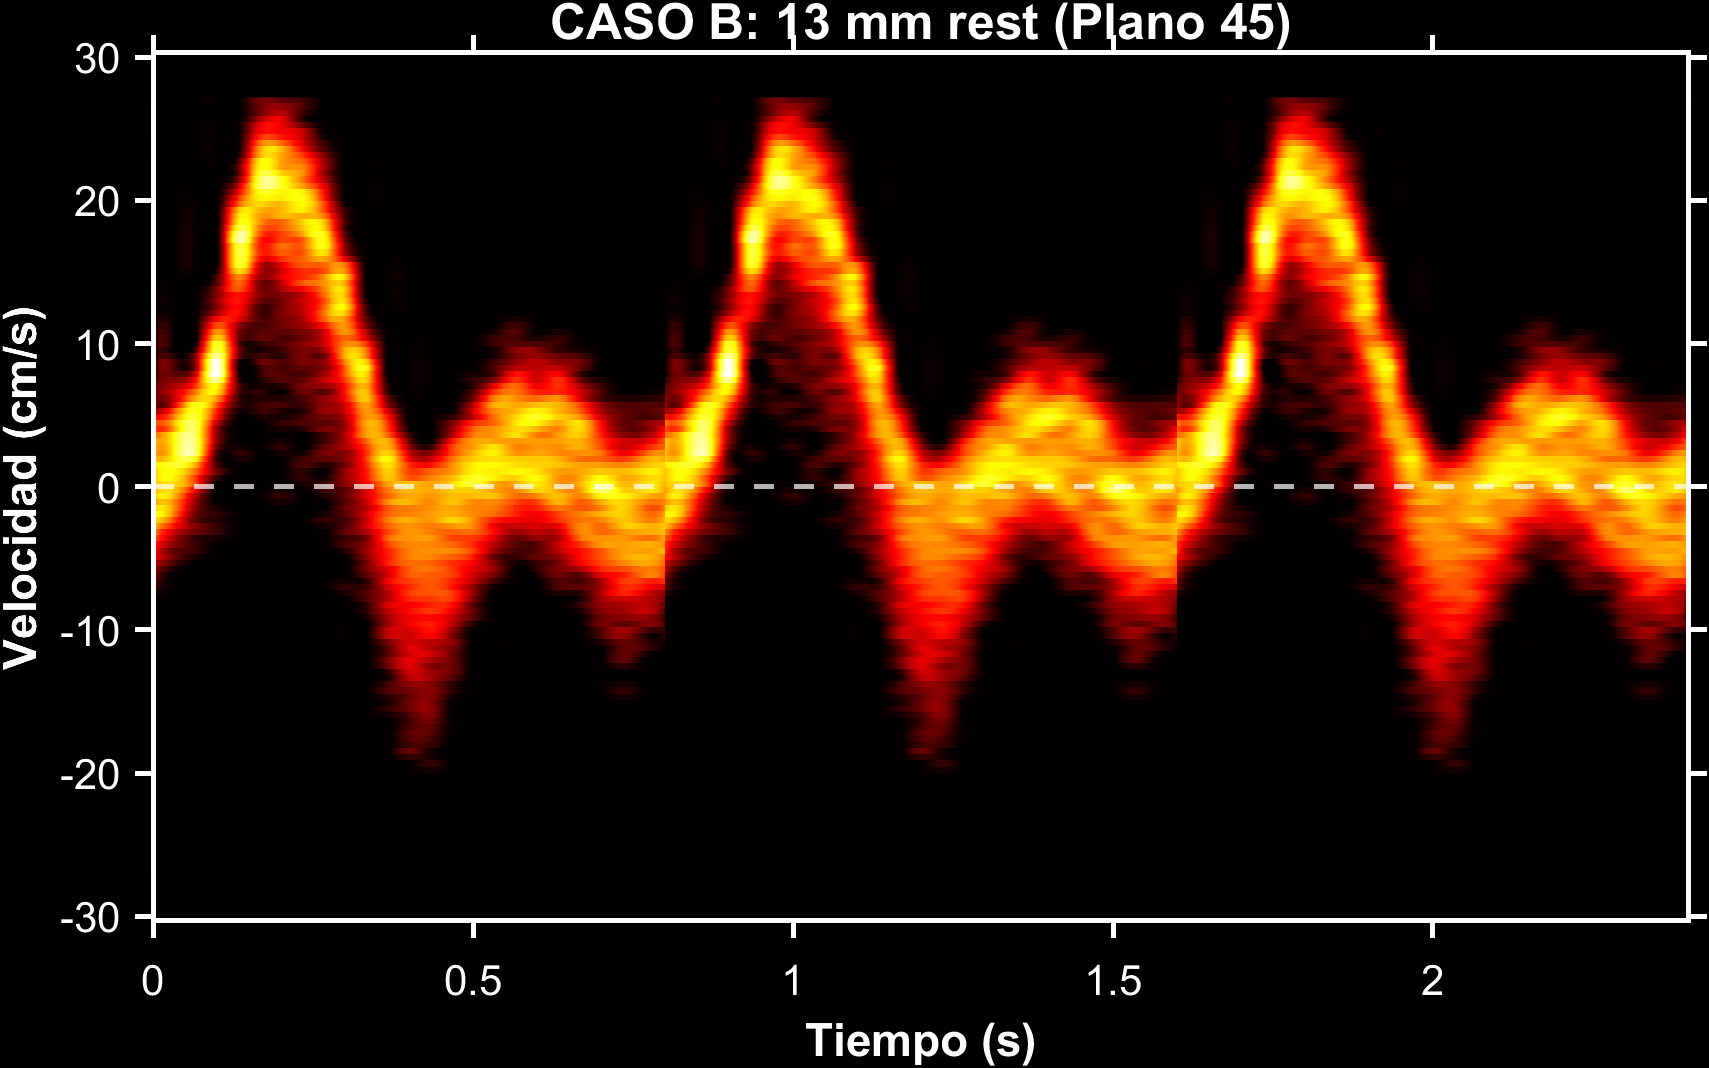
\includegraphics[width=\linewidth]{figures/anexos/13_mm_rest_Plano45.png}
            \caption{\href{https://drive.google.com/file/d/1LgYvr6ug48dCXbW_NYl_JJqlRzGxxMOV/view?usp=sharing}{Fantoma 13 mm \textbf{(Escuchar)}}}
            \label{fig:anexo_p45_13mm}
        \end{subfigure}
        
        \vspace{0.4cm}
        
        \begin{subfigure}{0.48\linewidth}
            \centering
            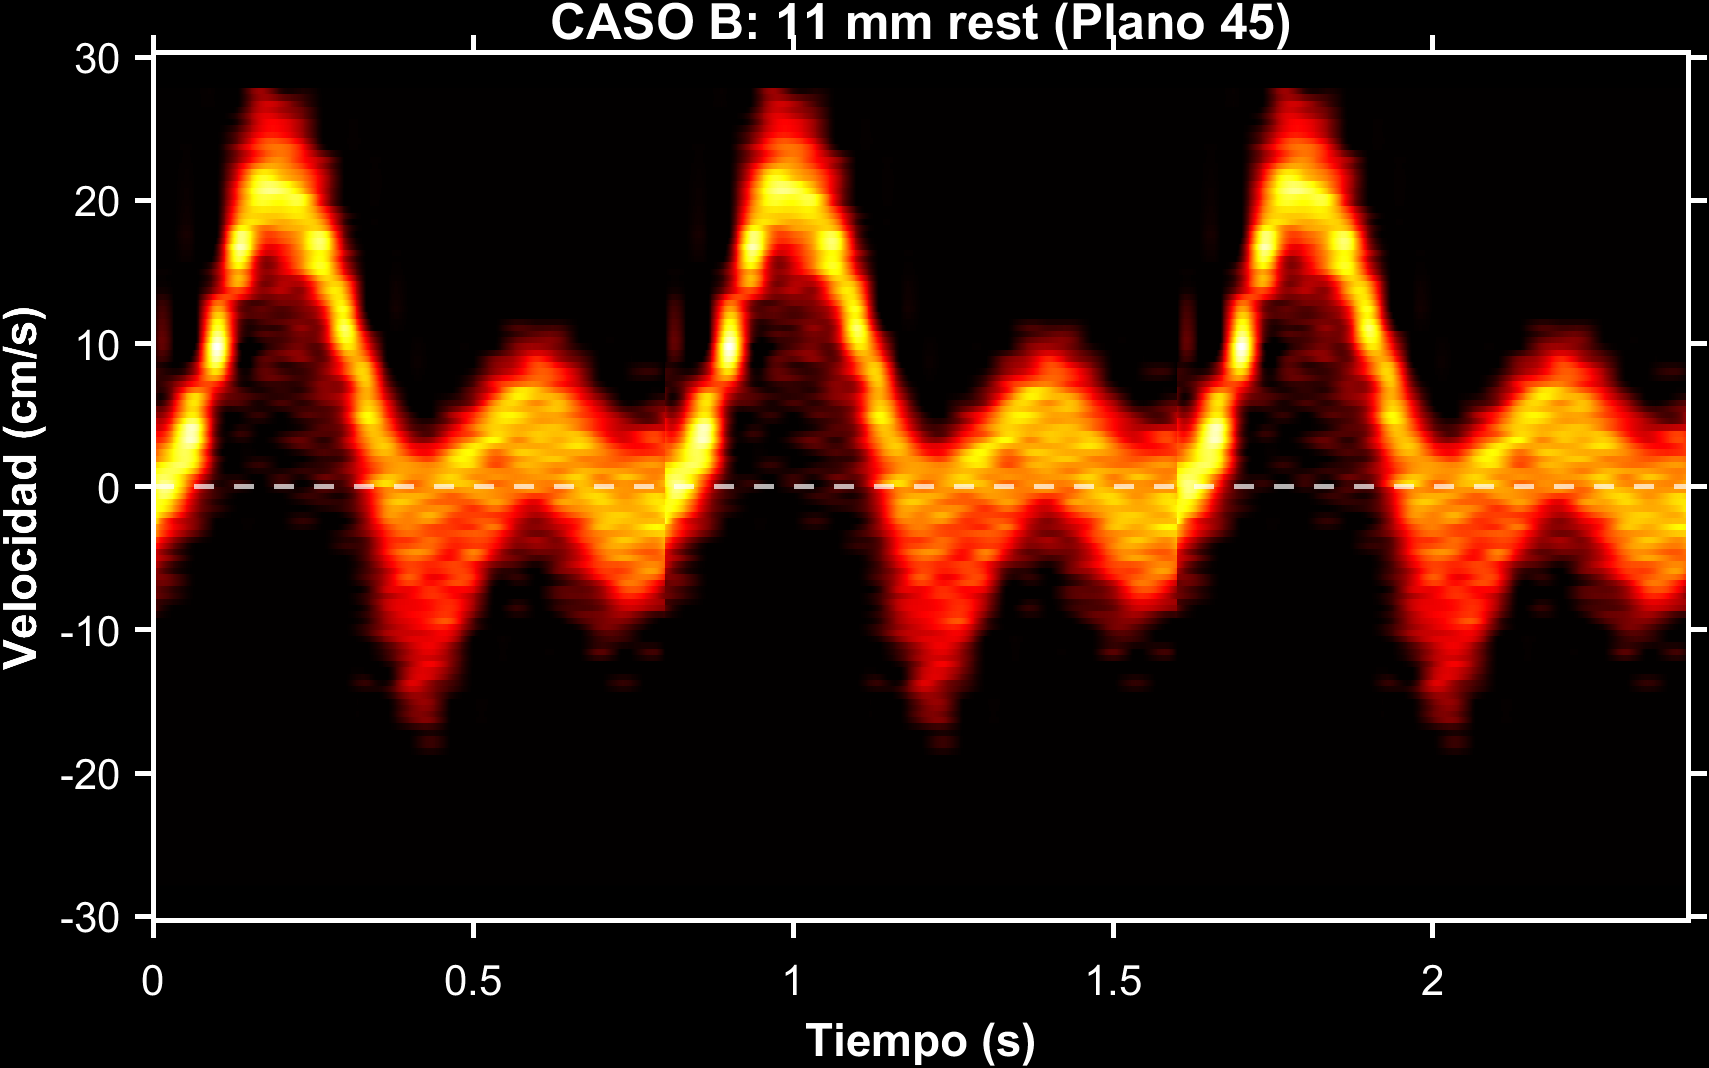
\includegraphics[width=\linewidth]{figures/anexos/11_mm_rest_Plano45.png}
            \caption{\href{https://drive.google.com/file/d/13VOYyAe2TLGDEpzZFB-JEHpD3smXe__b/view?usp=sharing}{Fantoma 11 mm \textbf{(Escuchar)}}}
            \label{fig:anexo_p45_11mm}
        \end{subfigure}\hfill
        \begin{subfigure}{0.48\linewidth}
            \centering
            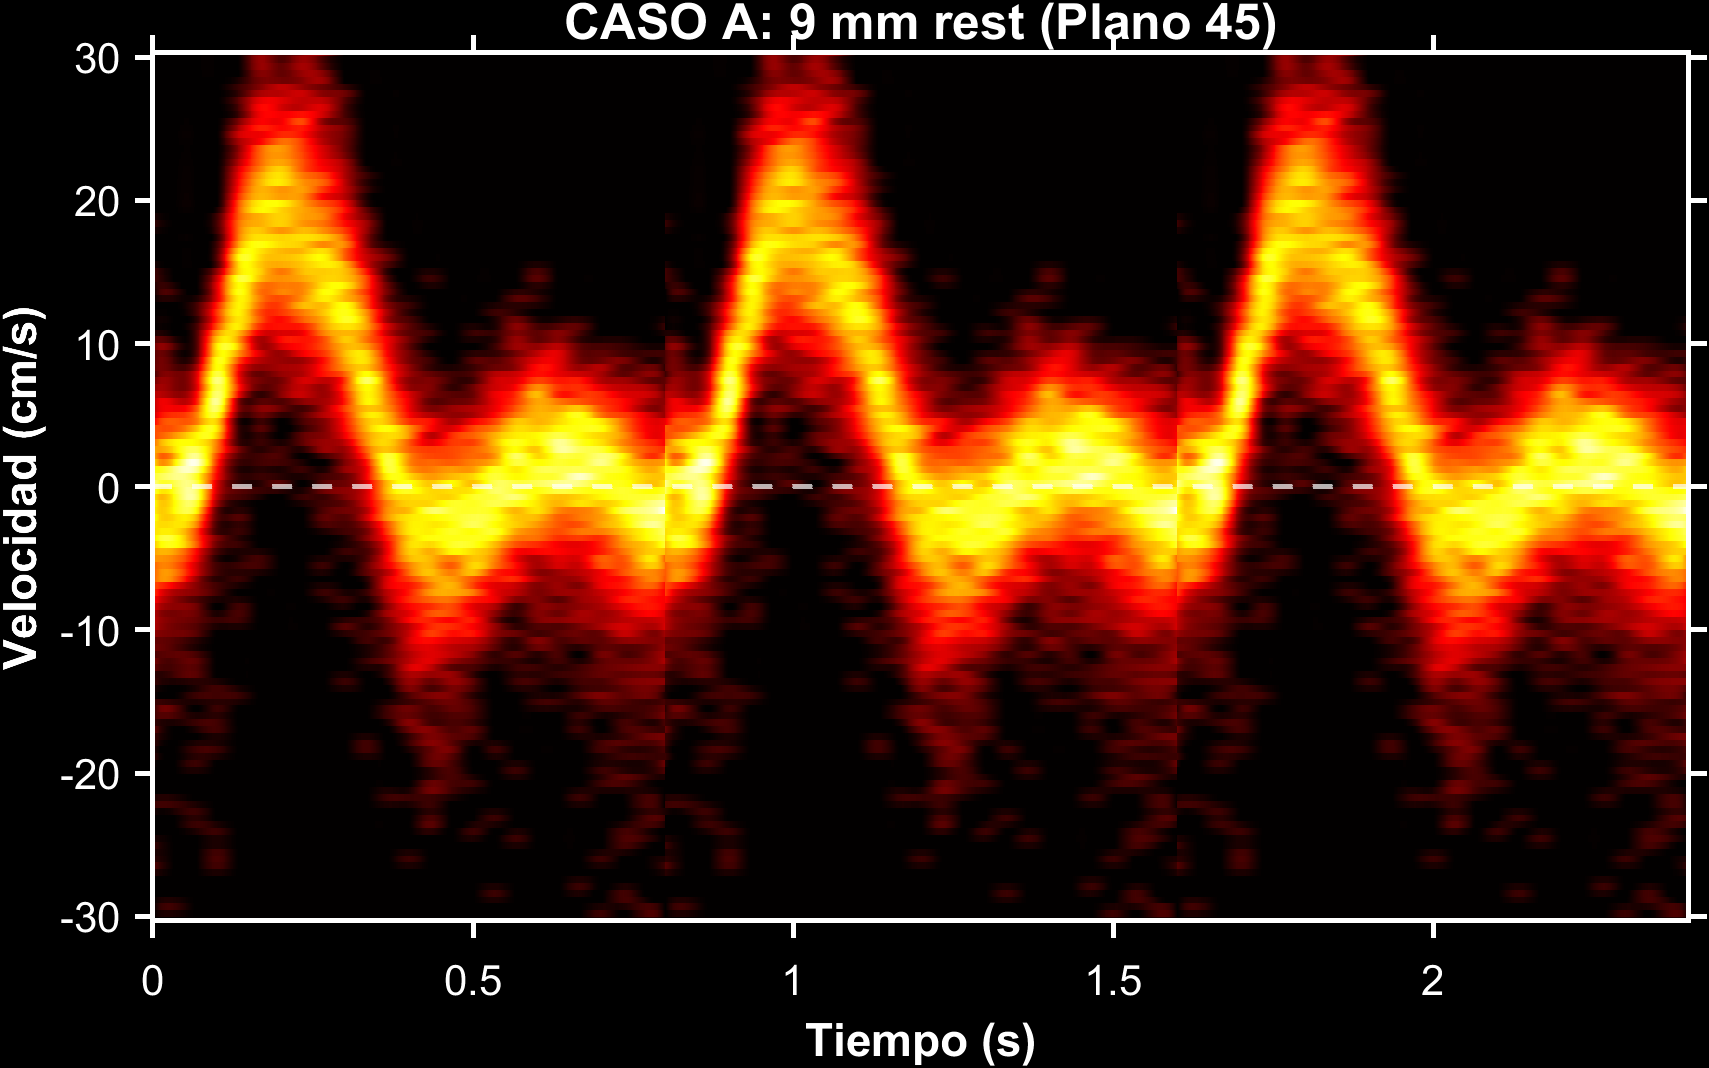
\includegraphics[width=\linewidth]{figures/anexos/9_mm_rest_Plano45.png}
            \caption{\href{https://drive.google.com/file/d/1a5bmth4i0mA5p9IGHgH1vpA63KkmTlW6/view?usp=sharing}{Fantoma 9 mm \textbf{(Escuchar)}}}
            \label{fig:anexo_p45_9mm}
        \end{subfigure}
    \end{minipage}
    \caption{\label{fig:anexo_comparacion_p45}Evolución espectral en la zona del arco aórtico bajo condición de reposo. Fuente: Elaboración propia.}
\end{figure}


\subsection{Análisis comparativo: Pre-coartación (plano 53)}

\begin{figure}[H]
    \centering
    \begin{minipage}{0.75\textwidth}
        \begin{subfigure}{0.48\linewidth}
            \centering
            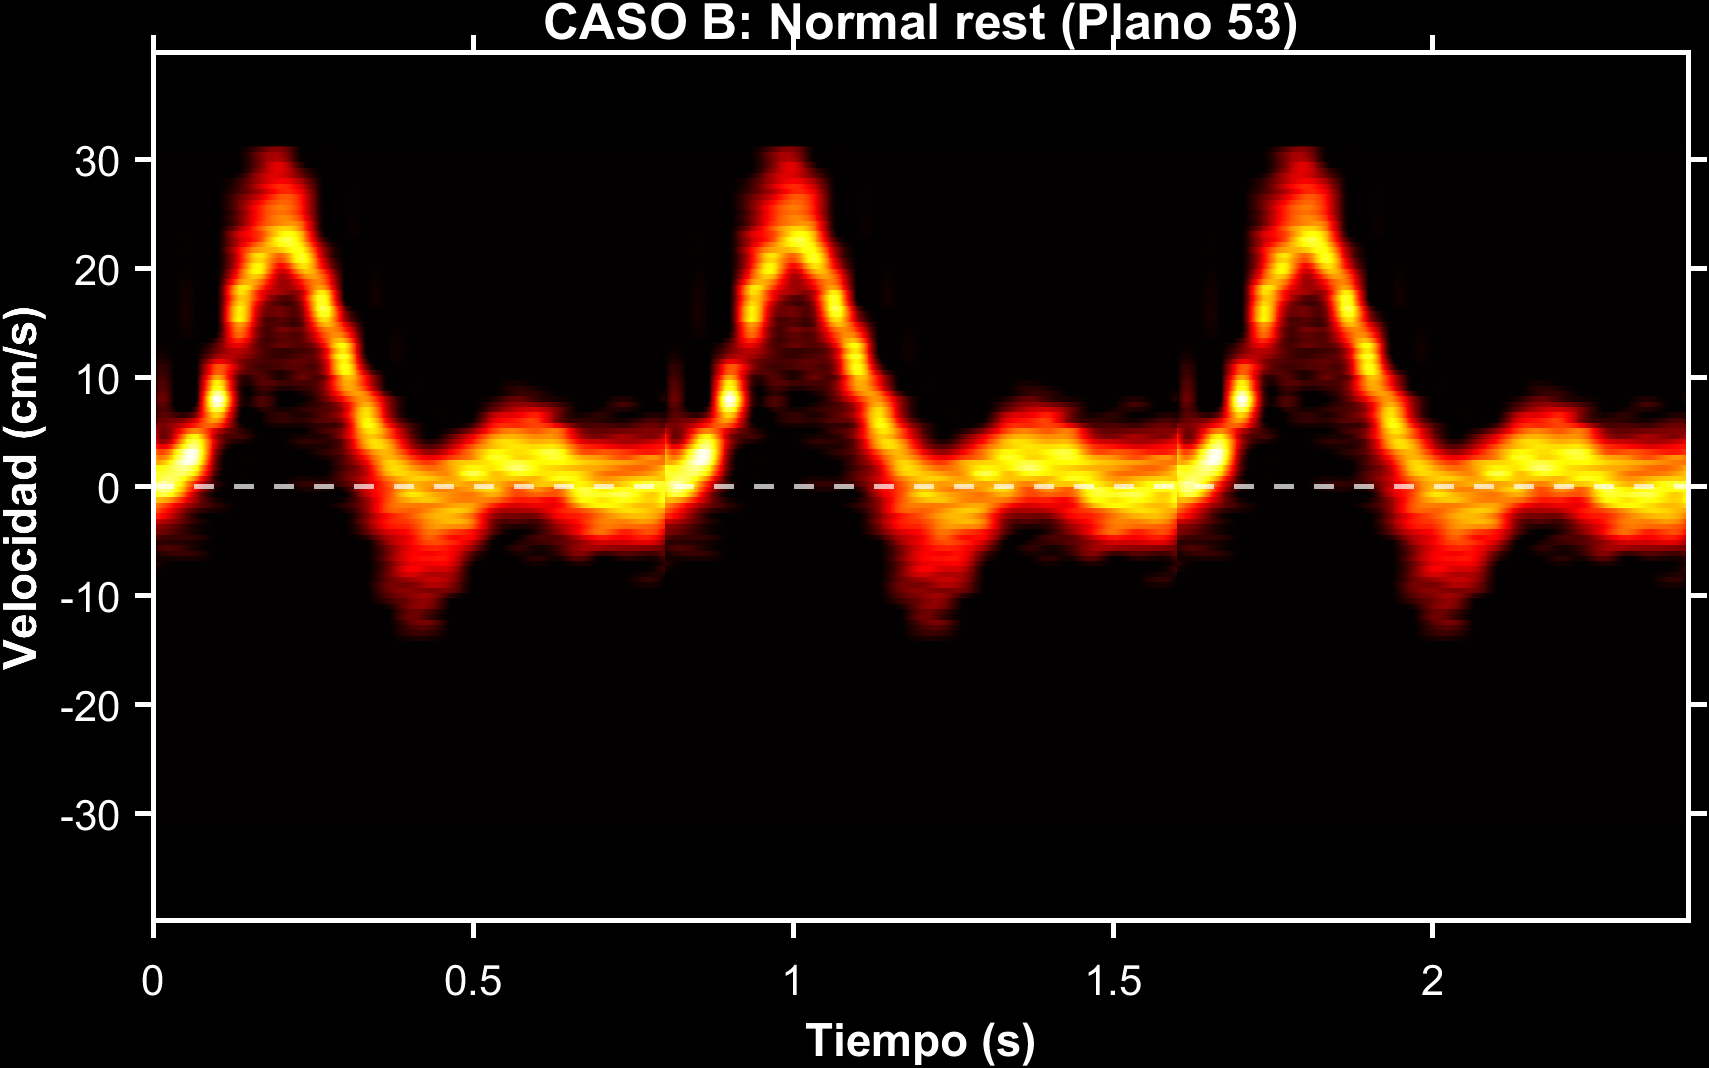
\includegraphics[width=\linewidth]{figures/anexos/Normal_rest_Plano53.png}
            \caption{\href{https://drive.google.com/file/d/1HOFjscXZdn0Xqr6QBVaSOorMYazGTOI1/view?usp=sharing}{Fantoma normal \textbf{(Escuchar)}}}
            \label{fig:anexo_p53_normal}
        \end{subfigure}\hfill
        \begin{subfigure}{0.48\linewidth}
            \centering
            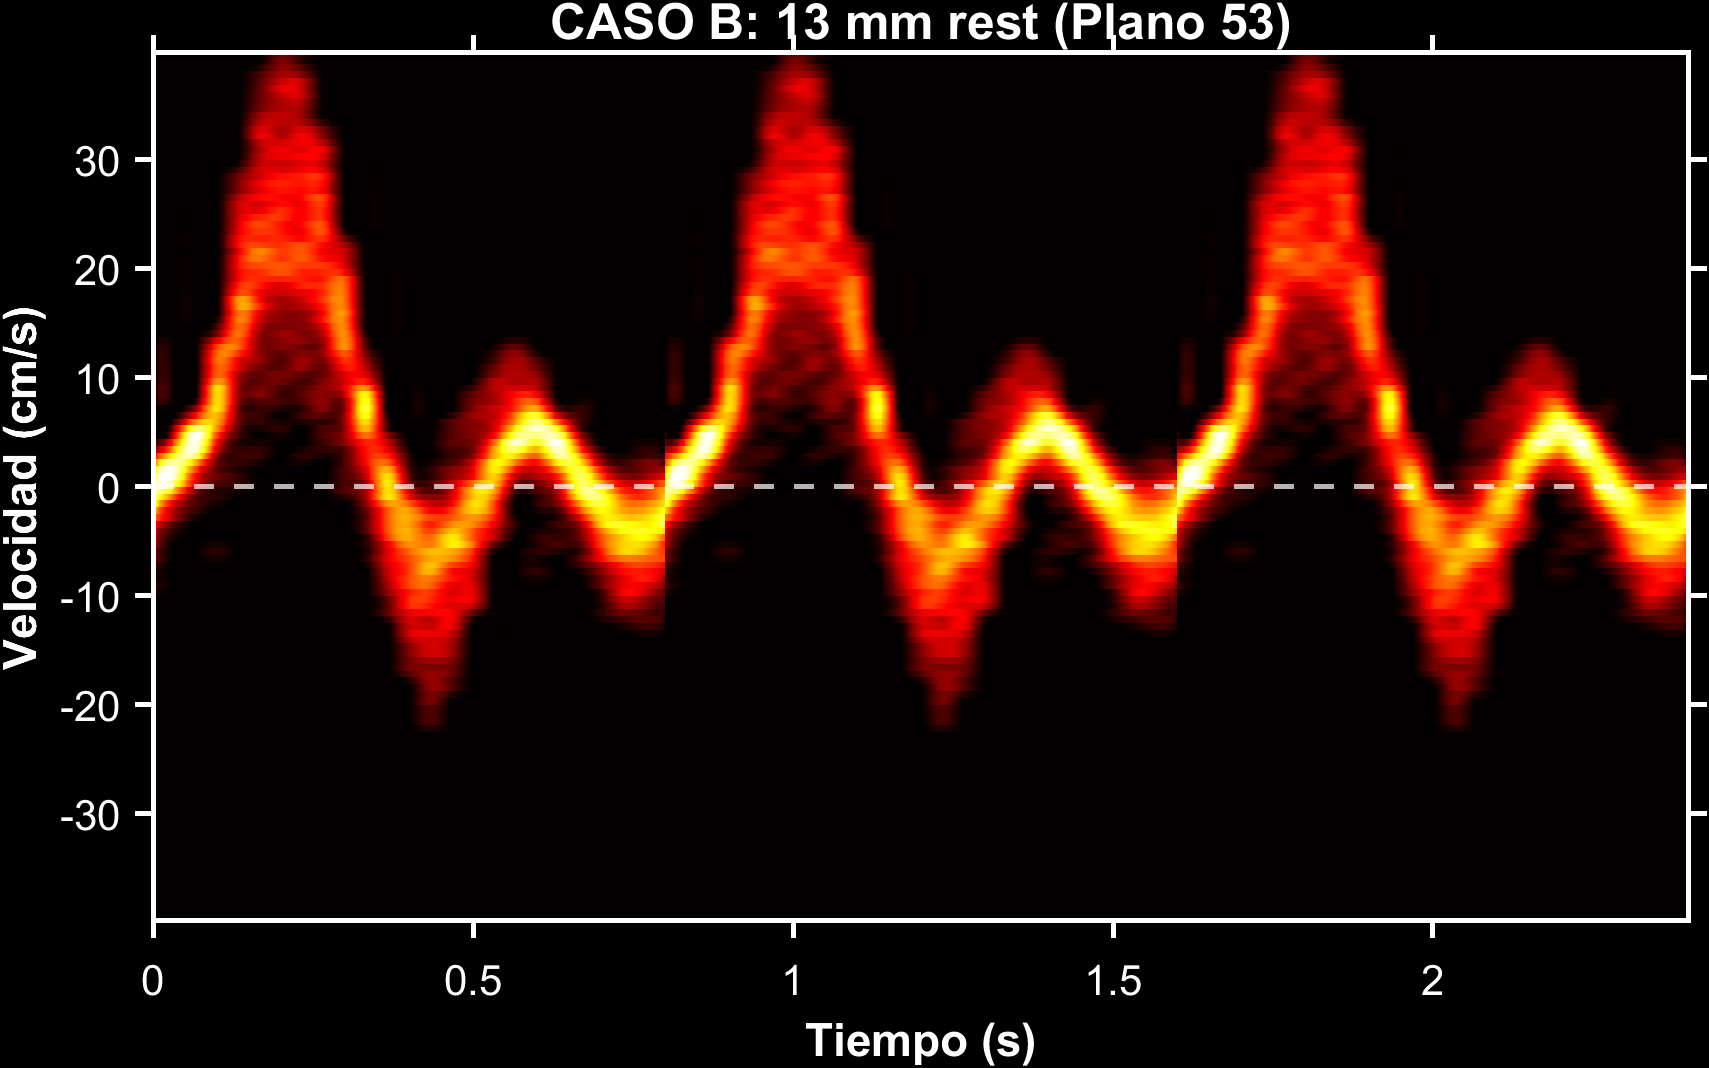
\includegraphics[width=\linewidth]{figures/anexos/13_mm_rest_Plano53.png}
            \caption{\href{https://drive.google.com/file/d/13ViBrWH2iWedRAWQrjs2DRwnu1cg7DFN/view?usp=sharing}{Fantoma 13 mm \textbf{(Escuchar)}}}
            \label{fig:anexo_p53_13mm}
        \end{subfigure}
        
        \vspace{0.4cm}
        
        \begin{subfigure}{0.48\linewidth}
            \centering
            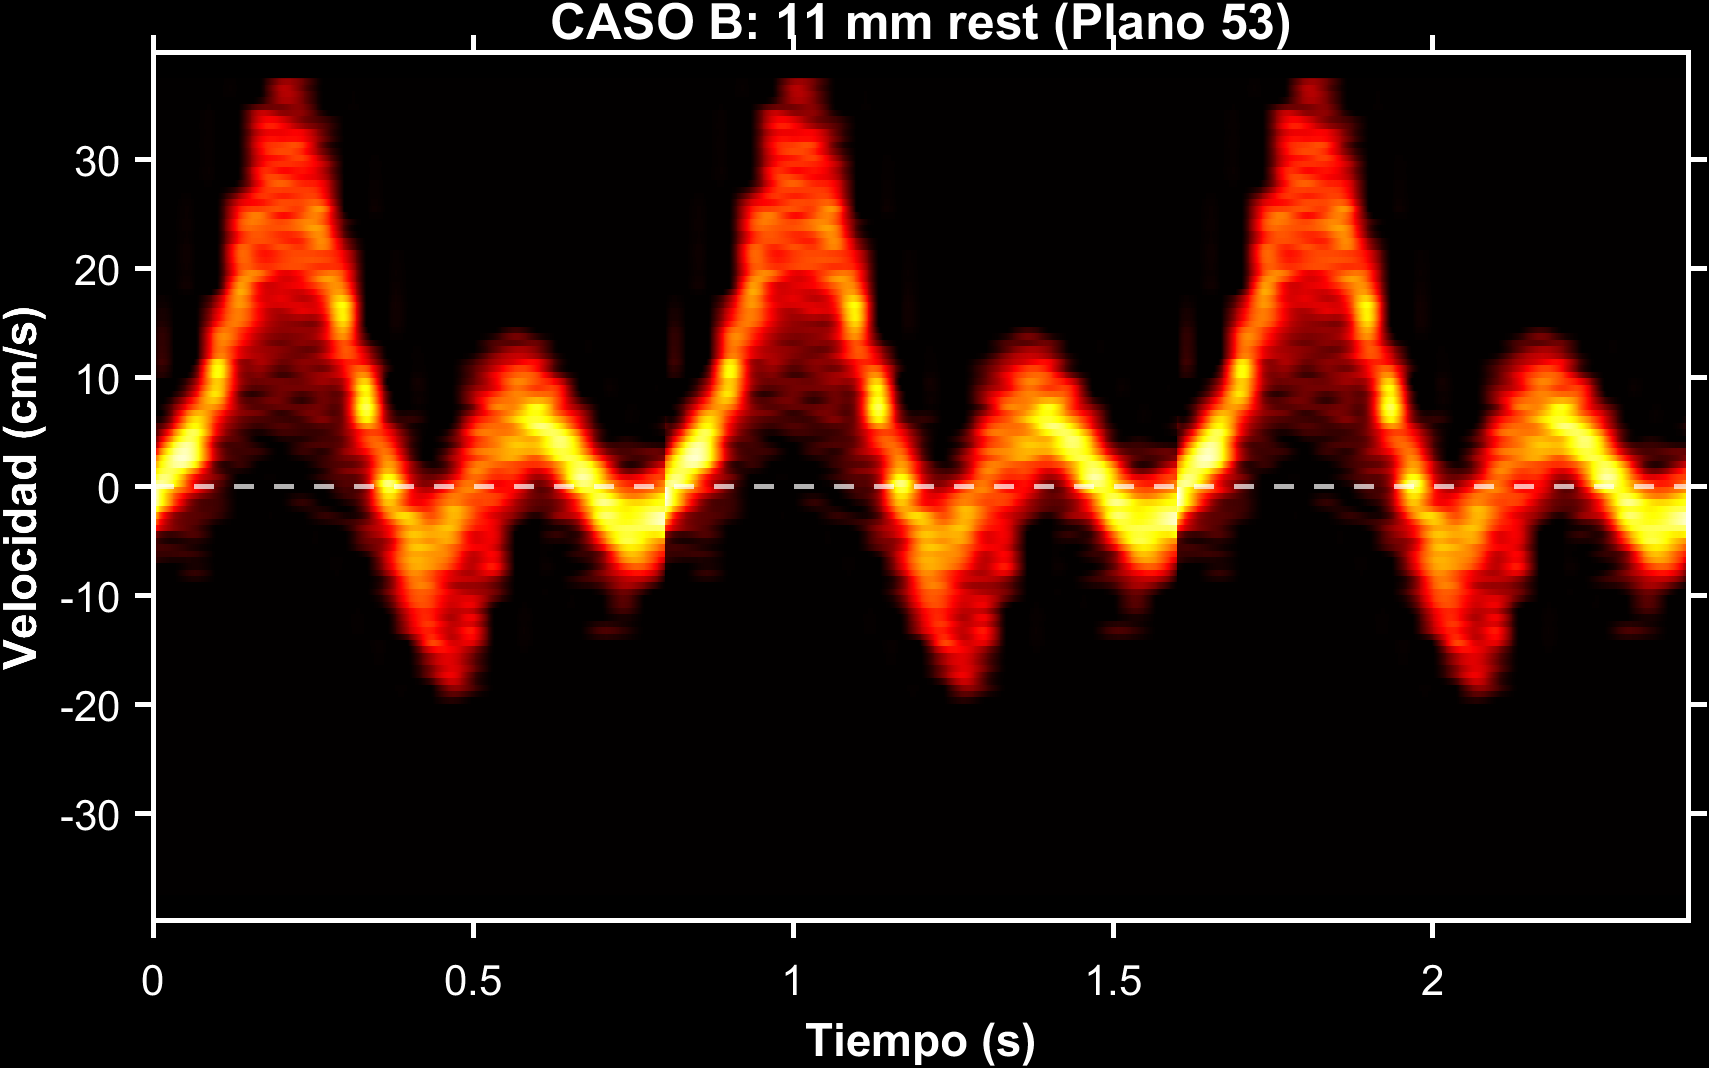
\includegraphics[width=\linewidth]{figures/anexos/11_mm_rest_Plano53.png}
            \caption{\href{https://drive.google.com/file/d/1gsotKFrU7cHhEvFR5qXwZjdcTrV017aL/view?usp=sharing}{Fantoma 11 mm \textbf{(Escuchar)}}}
            \label{fig:anexo_p53_11mm}
        \end{subfigure}\hfill
        \begin{subfigure}{0.48\linewidth}
            \centering
            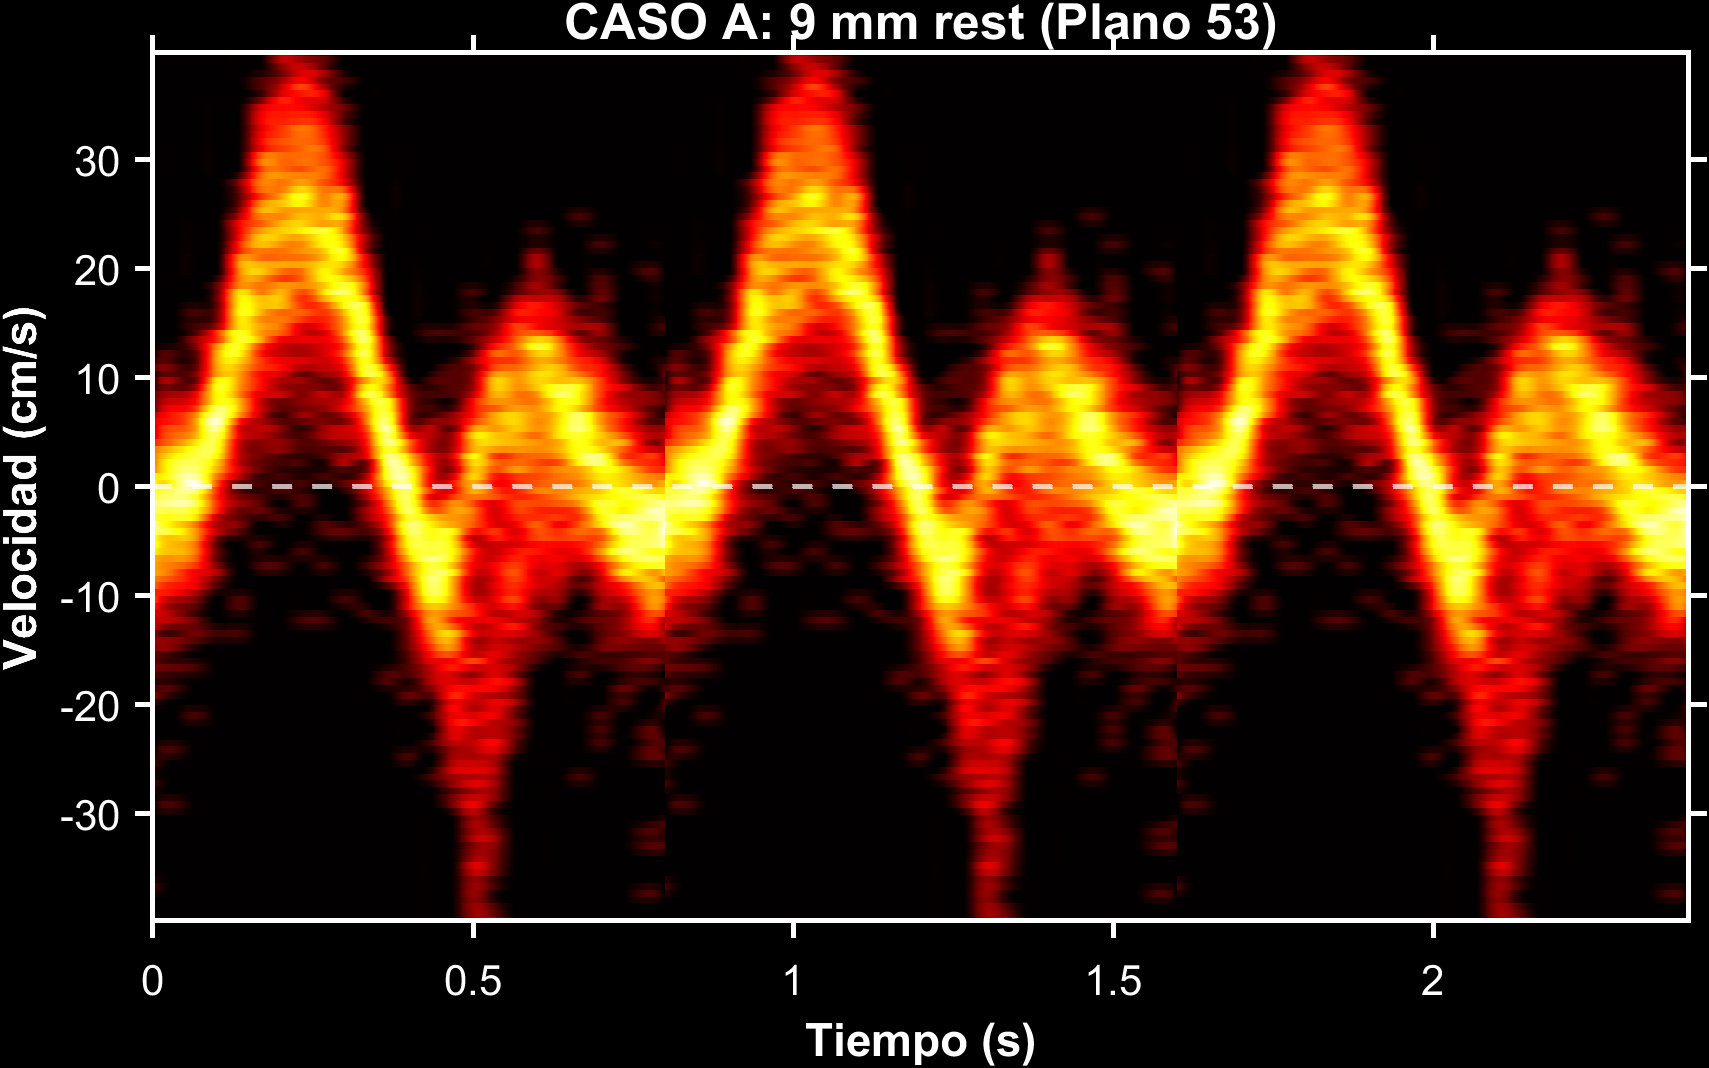
\includegraphics[width=\linewidth]{figures/anexos/9_mm_rest_Plano53.png}
            \caption{\href{https://drive.google.com/file/d/1iDhg9IqTgnRclAD8EpGDnmnlDcU6DA5I/view?usp=sharing}{Fantoma 9 mm \textbf{(Escuchar)}}}
            \label{fig:anexo_p53_9mm}
        \end{subfigure}
    \end{minipage}
    \caption{\label{fig:anexo_comparacion_p53} Evolución espectral en la zona pre-coartación bajo condición de reposo. Fuente: Elaboración propia.}
\end{figure}


\subsection{Análisis comparativo: Post-coartación (plano 70)}

\begin{figure}[H]
    \centering
    \begin{minipage}{0.75\textwidth}
        \begin{subfigure}{0.48\linewidth}
            \centering
            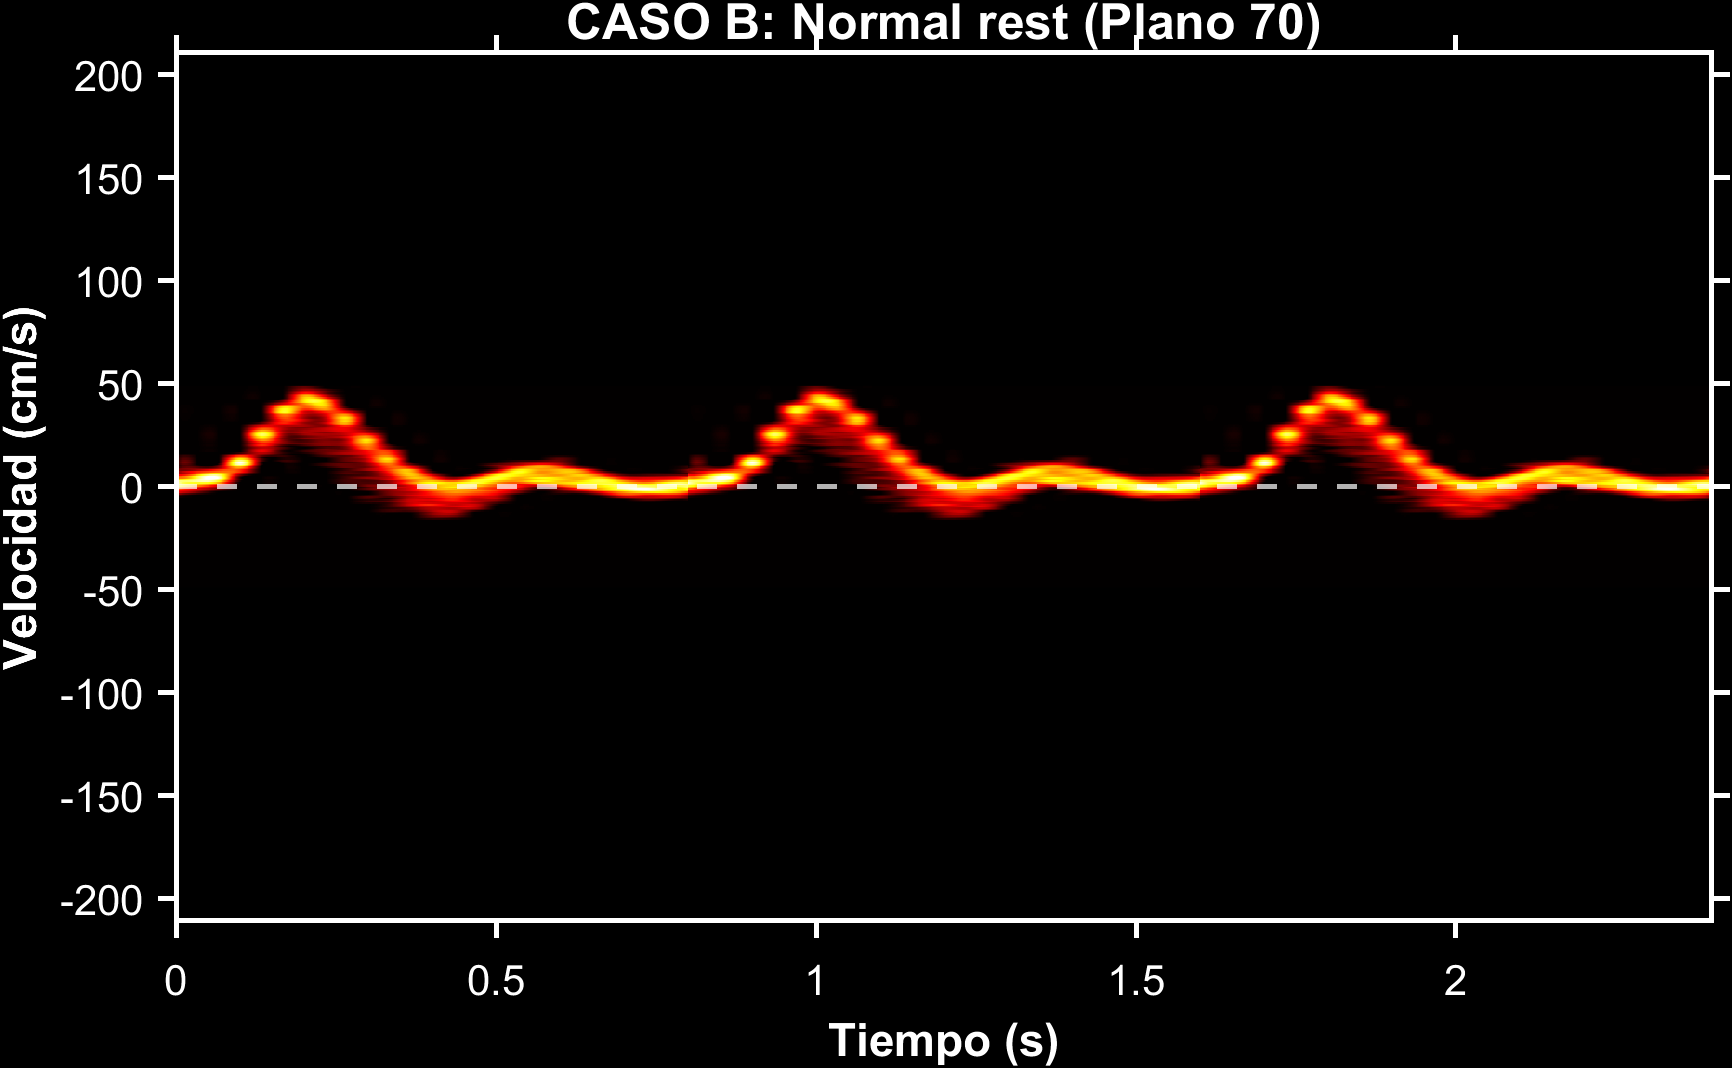
\includegraphics[width=\linewidth]{figures/anexos/Normal_rest_Plano70.png}
            \caption{\href{https://drive.google.com/file/d/1Ji-aclVUsA0XJH64ZcgiSzRloFJDtPAL/view?usp=sharing}{Fantoma normal \textbf{(Escuchar)}}}
            \label{fig:anexo_p70_normal}
        \end{subfigure}\hfill
        \begin{subfigure}{0.48\linewidth}
            \centering
            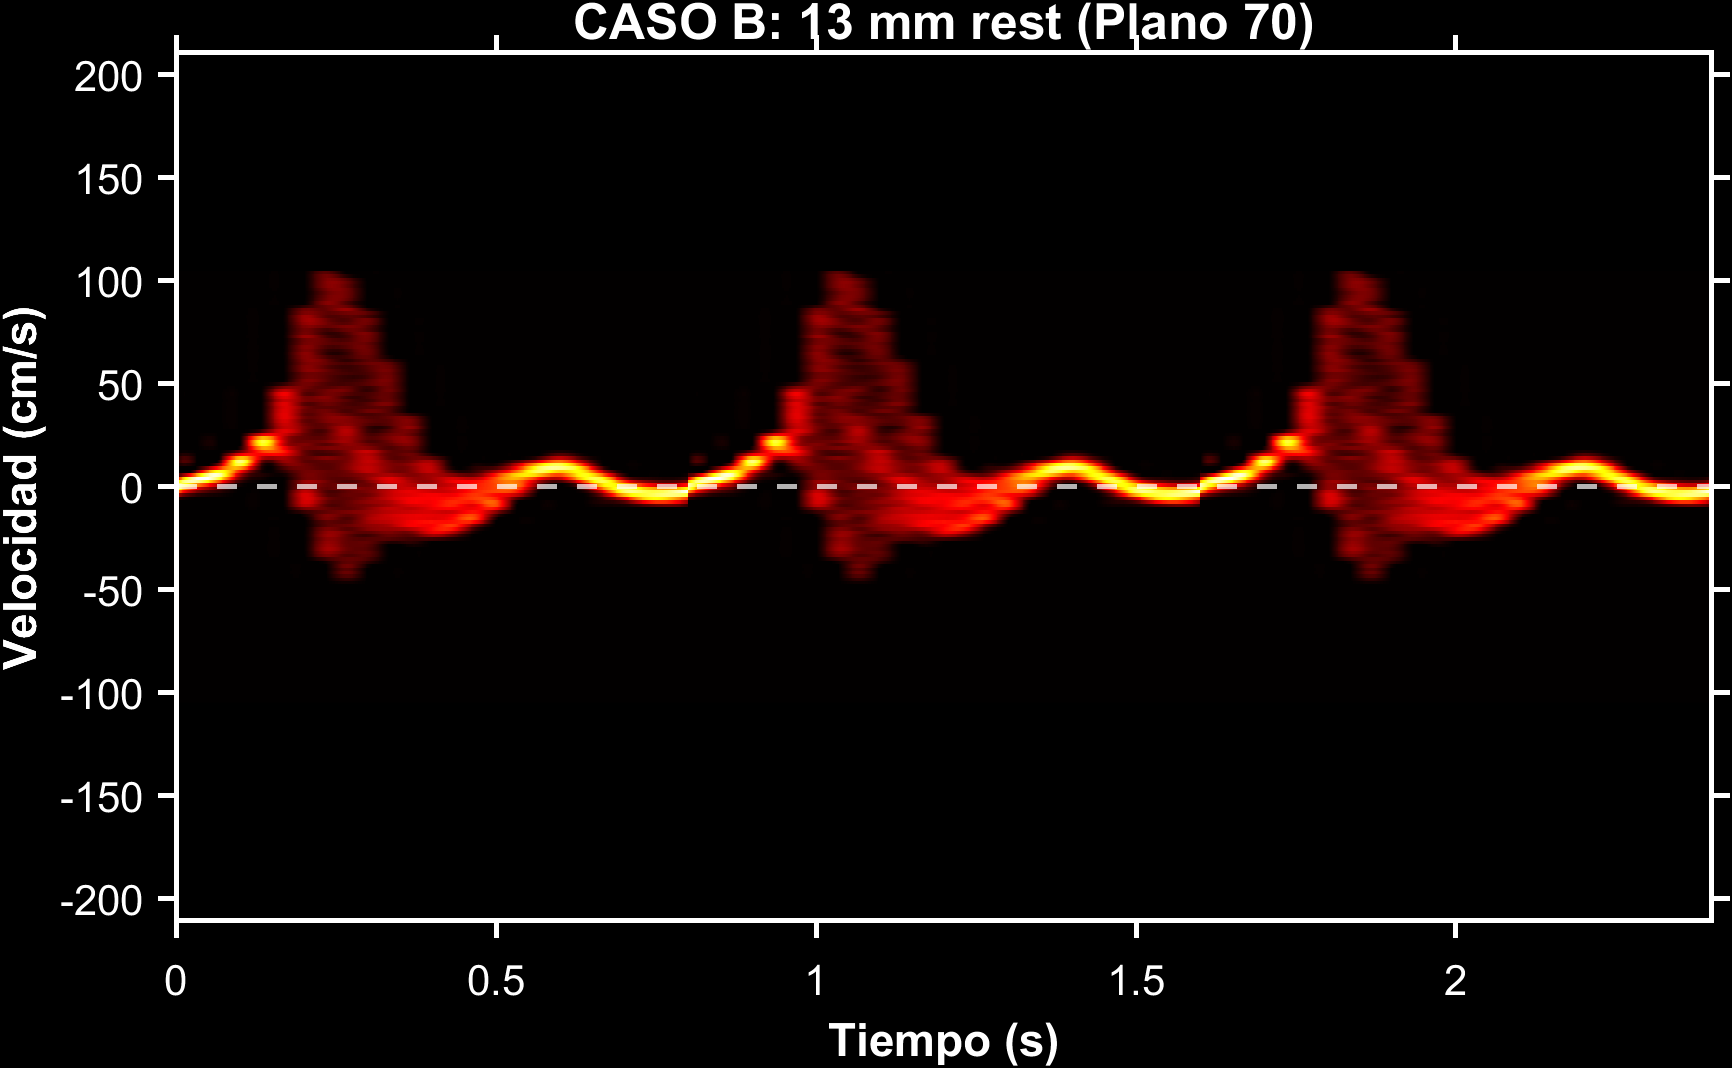
\includegraphics[width=\linewidth]{figures/anexos/13_mm_rest_Plano70.png}
            \caption{\href{https://drive.google.com/file/d/1BXh4fTabW4XNHS3mBkfjZjcfltDJDK9o/view?usp=sharing}{Fantoma 13 mm \textbf{(Escuchar)}}}
            \label{fig:anexo_p70_13mm}
        \end{subfigure}
        
        \vspace{0.4cm}
        
        \begin{subfigure}{0.48\linewidth}
            \centering
            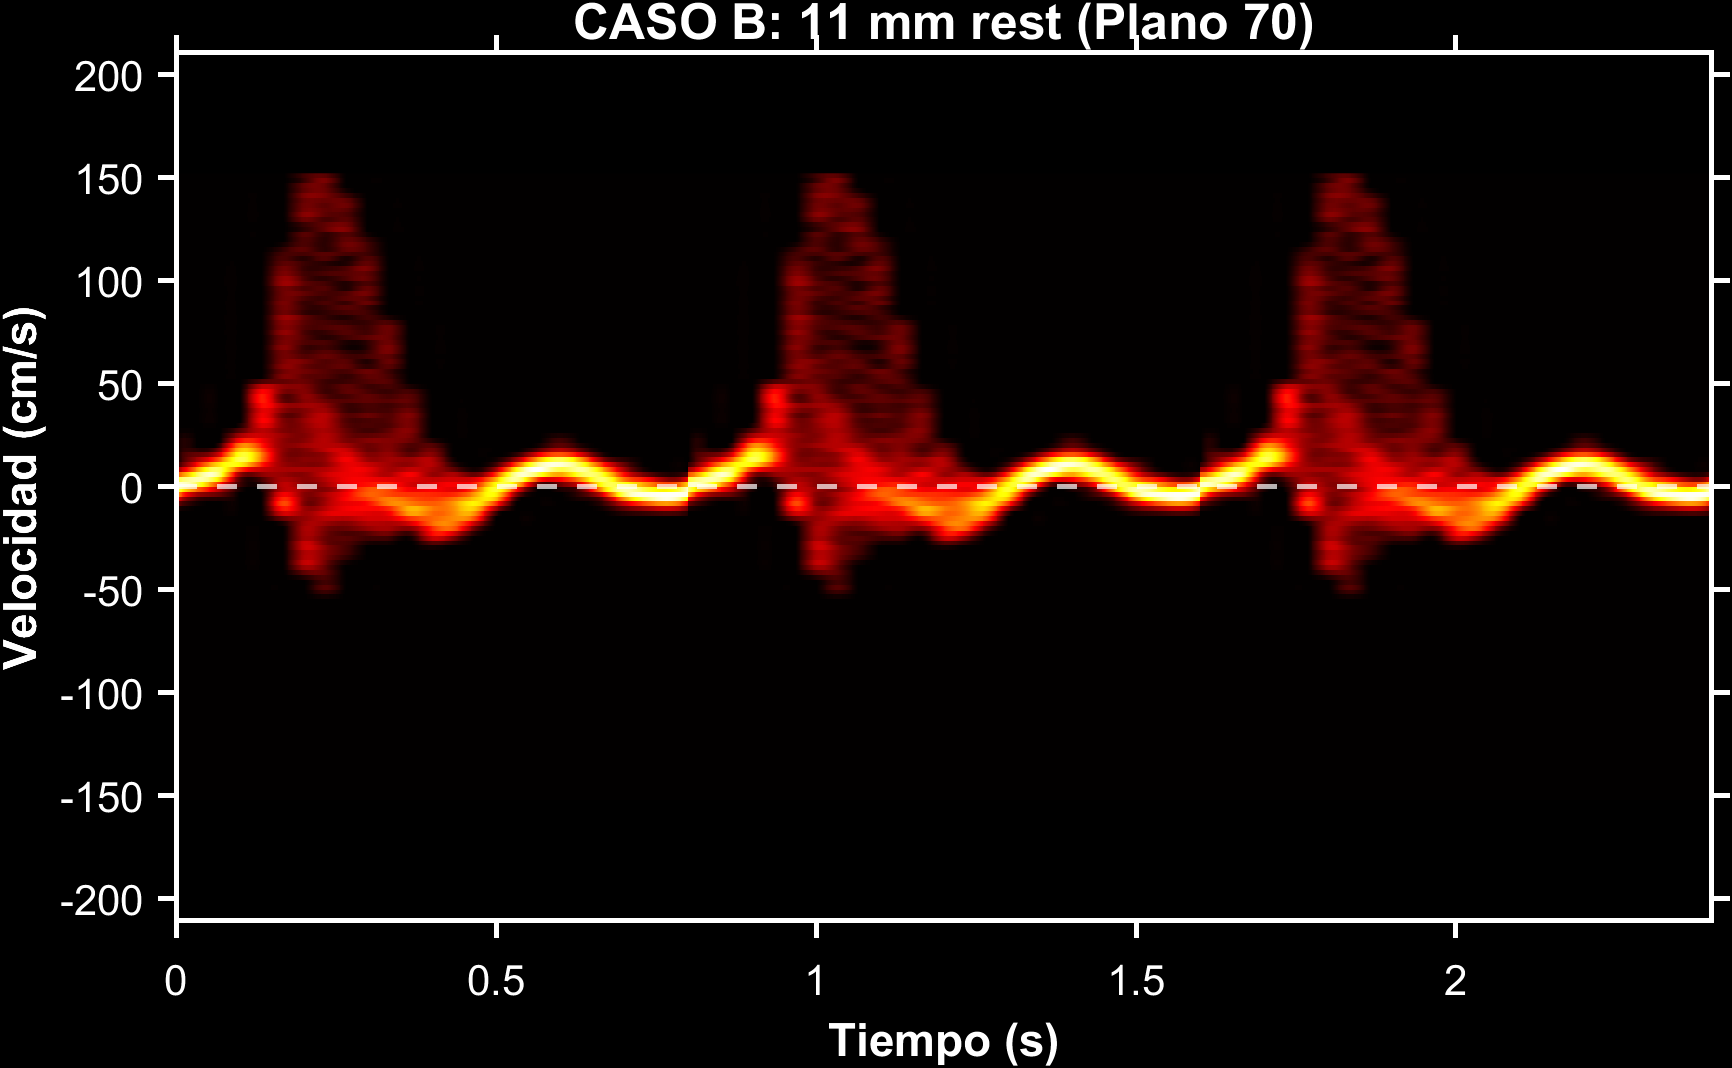
\includegraphics[width=\linewidth]{figures/anexos/11_mm_rest_Plano70.png}
            \caption{\href{https://drive.google.com/file/d/1vKdsexjQyZKzabsV51s44r13G063QVPx/view?usp=sharing}{Fantoma 11 mm \textbf{(Escuchar)}}}
            \label{fig:anexo_p70_11mm}
        \end{subfigure}\hfill
        \begin{subfigure}{0.48\linewidth}
            \centering
            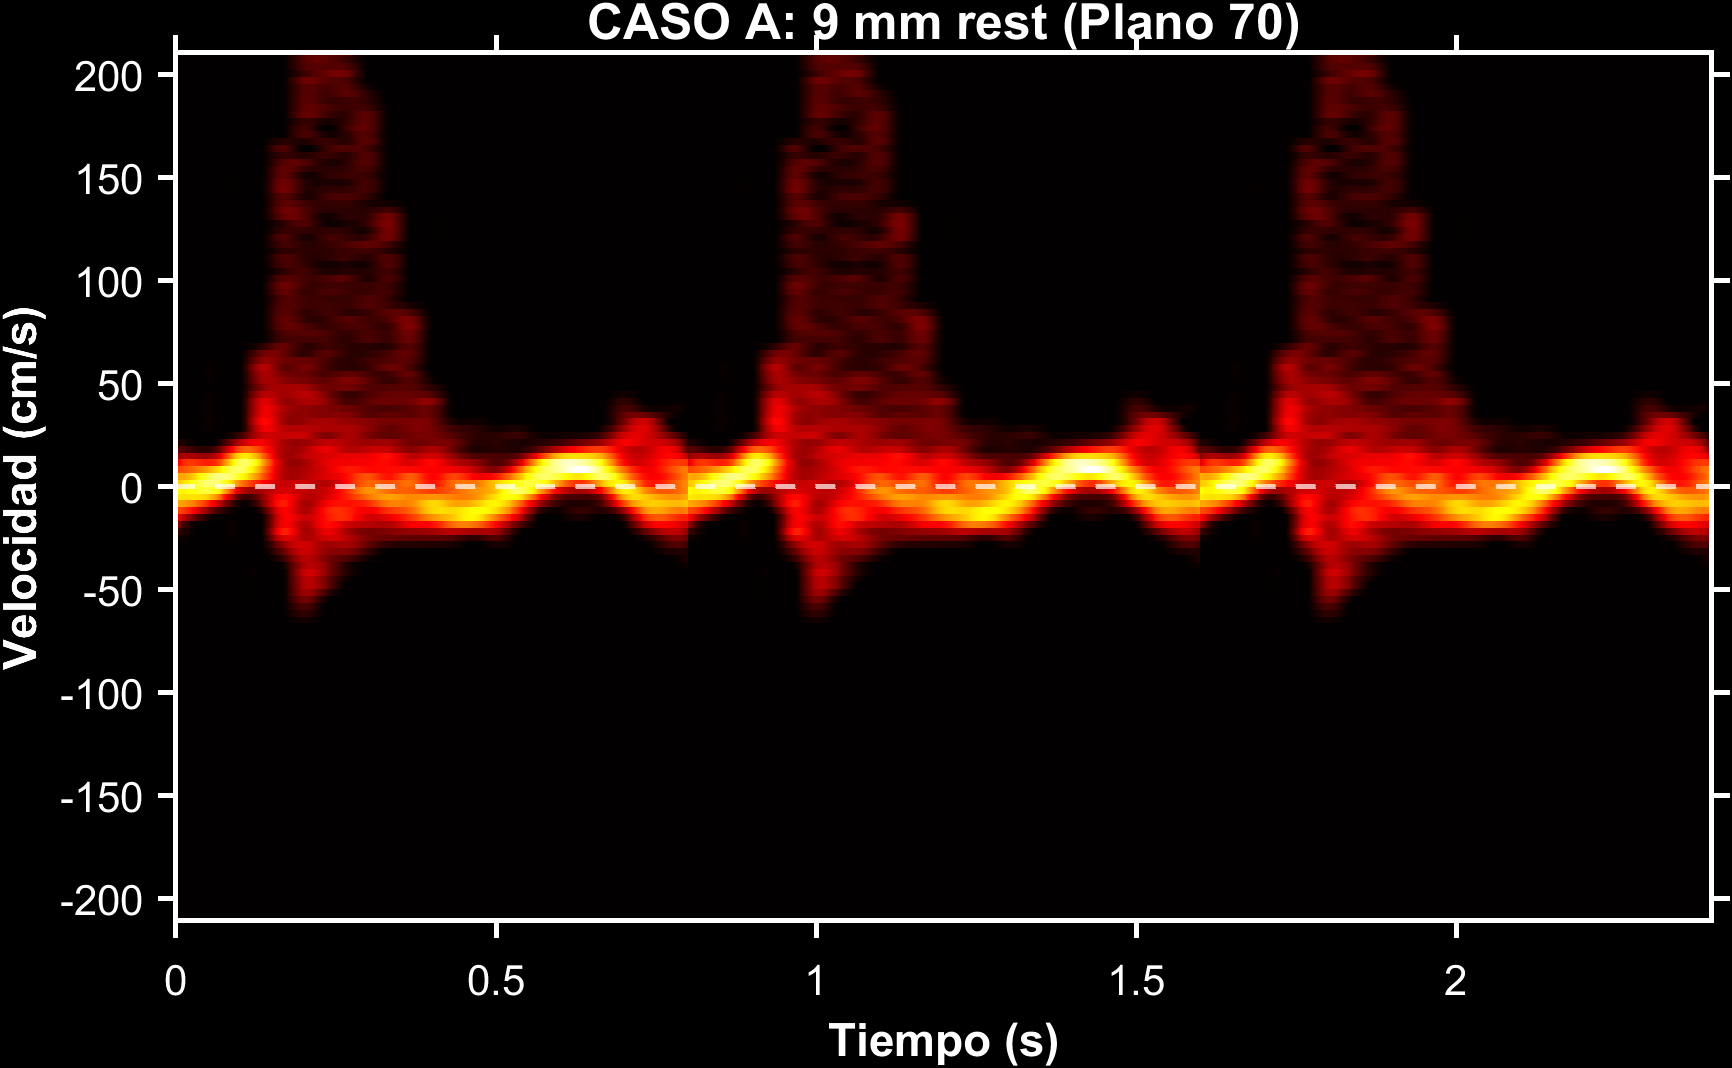
\includegraphics[width=\linewidth]{figures/anexos/9_mm_rest_Plano70.png}
            \caption{\href{https://drive.google.com/file/d/1aBgqeoV4qCd36aoZfs8mPQ5ol-GI3i1W/view?usp=sharing}{Fantoma 9 mm \textbf{(Escuchar)}}}
            \label{fig:anexo_p70_9mm}
        \end{subfigure}
    \end{minipage}
    \caption{\label{fig:anexo_comparacion_p70} Evolución espectral en la zona post-coartación bajo condición de reposo. Fuente: Elaboración propia.}
\end{figure}

\section{Exploración de los casos borde}
\label{anexo:casos_borde}
En este anexo se presentan los casos borde de la segmentacion. Se incluyen las condiciones de reposo y estrés, para los fantomas normal y 9 mm. Para mantener la coherencia se presentan la geometría asociada y los diferentes planos.

\begin{figure}[H]
    \centering
    \begin{minipage}{0.75\textwidth}
        \begin{subfigure}{0.48\linewidth}
            \centering
            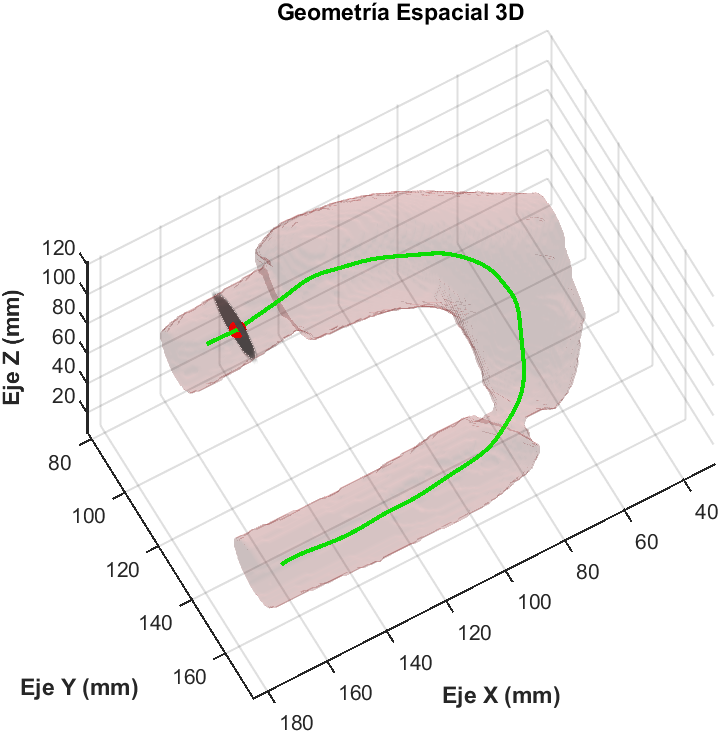
\includegraphics[width=\linewidth]{figures/anexos/9mm_plano5.png}
            \caption{Plano 5 (aorta ascendente proximal)}
            \label{fig:anexo_geo_p5}
        \end{subfigure}\hfill
        \begin{subfigure}{0.48\linewidth}
            \centering
            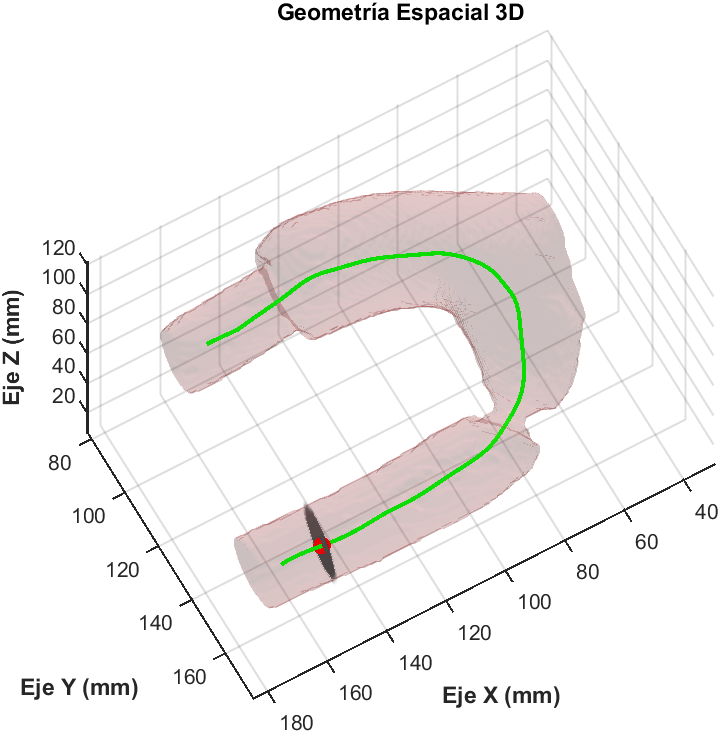
\includegraphics[width=\linewidth]{figures/anexos/9mm_plano85.png}
            \caption{Plano 85 (aorta descendente distal)}
            \label{fig:anexo_geo_p85}
        \end{subfigure}
    \end{minipage}
    \caption{\label{fig:anexo_geometria_extremos} Representación tridimensional del fantoma de 9mm. Ilustra la ubicación de los planos en los casos borde. La línea verde representa el \textit{centerline}. Fuente: Elaboración propia.}
\end{figure}

\subsection{Análisis comparativo extremo: Plano 5}

\begin{figure}[H]
    \centering
    \begin{minipage}{0.75\textwidth}
        \begin{subfigure}{0.48\linewidth}
            \centering
            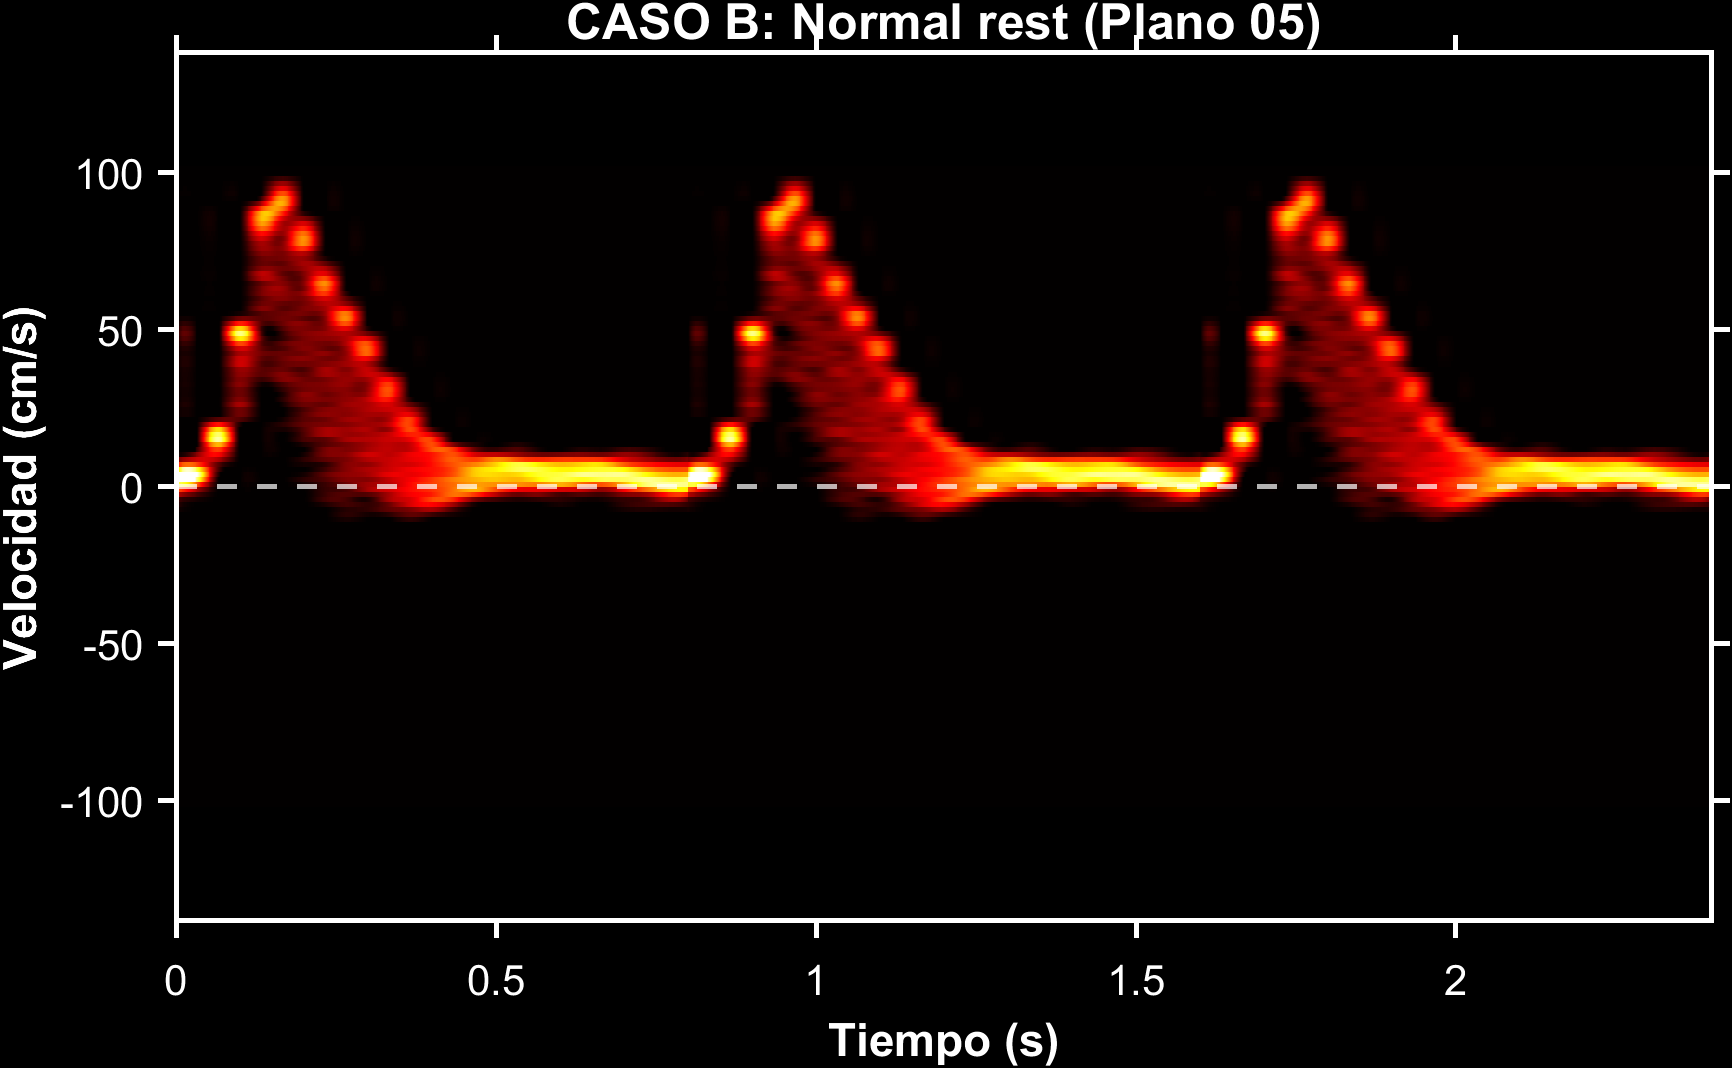
\includegraphics[width=\linewidth]{figures/anexos/Normal_rest_Plano05.png}
            \caption{\href{https://drive.google.com/file/d/1YK31lfkGaEXx60OxTx7NMA_Cw63nC900/view?usp=sharing}{Normal \textit{rest} \textbf{(Escuchar)}}}
            \label{fig:anexo_p5_normal_rest}
        \end{subfigure}\hfill
        \begin{subfigure}{0.48\linewidth}
            \centering
            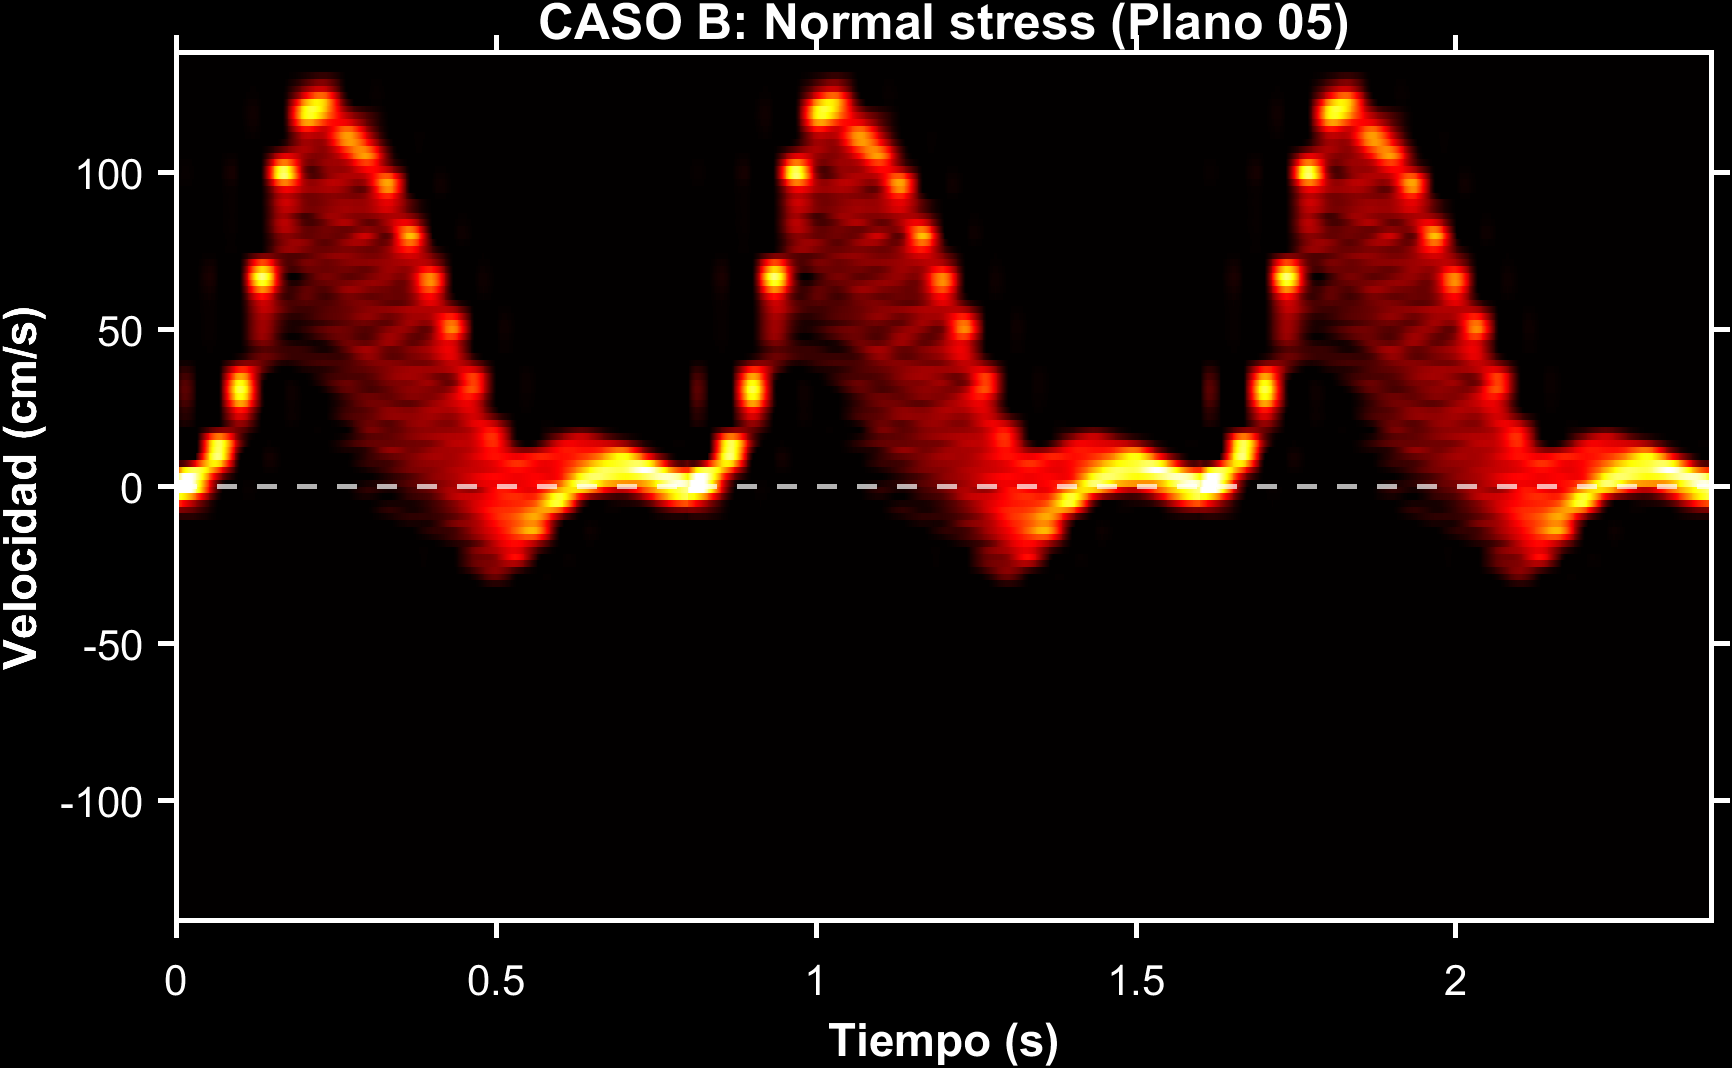
\includegraphics[width=\linewidth]{figures/anexos/Normal_stress_Plano05.png}
            \caption{\href{https://drive.google.com/file/d/1YZu0HmBU-EFEgWmTePQ66v50J-19i2o7/view?usp=sharing}{Normal \textit{stress} \textbf{(Escuchar)}}}
            \label{fig:anexo_p5_normal_stress}
        \end{subfigure}
        
        \vspace{0.4cm}
        
        \begin{subfigure}{0.48\linewidth}
            \centering
            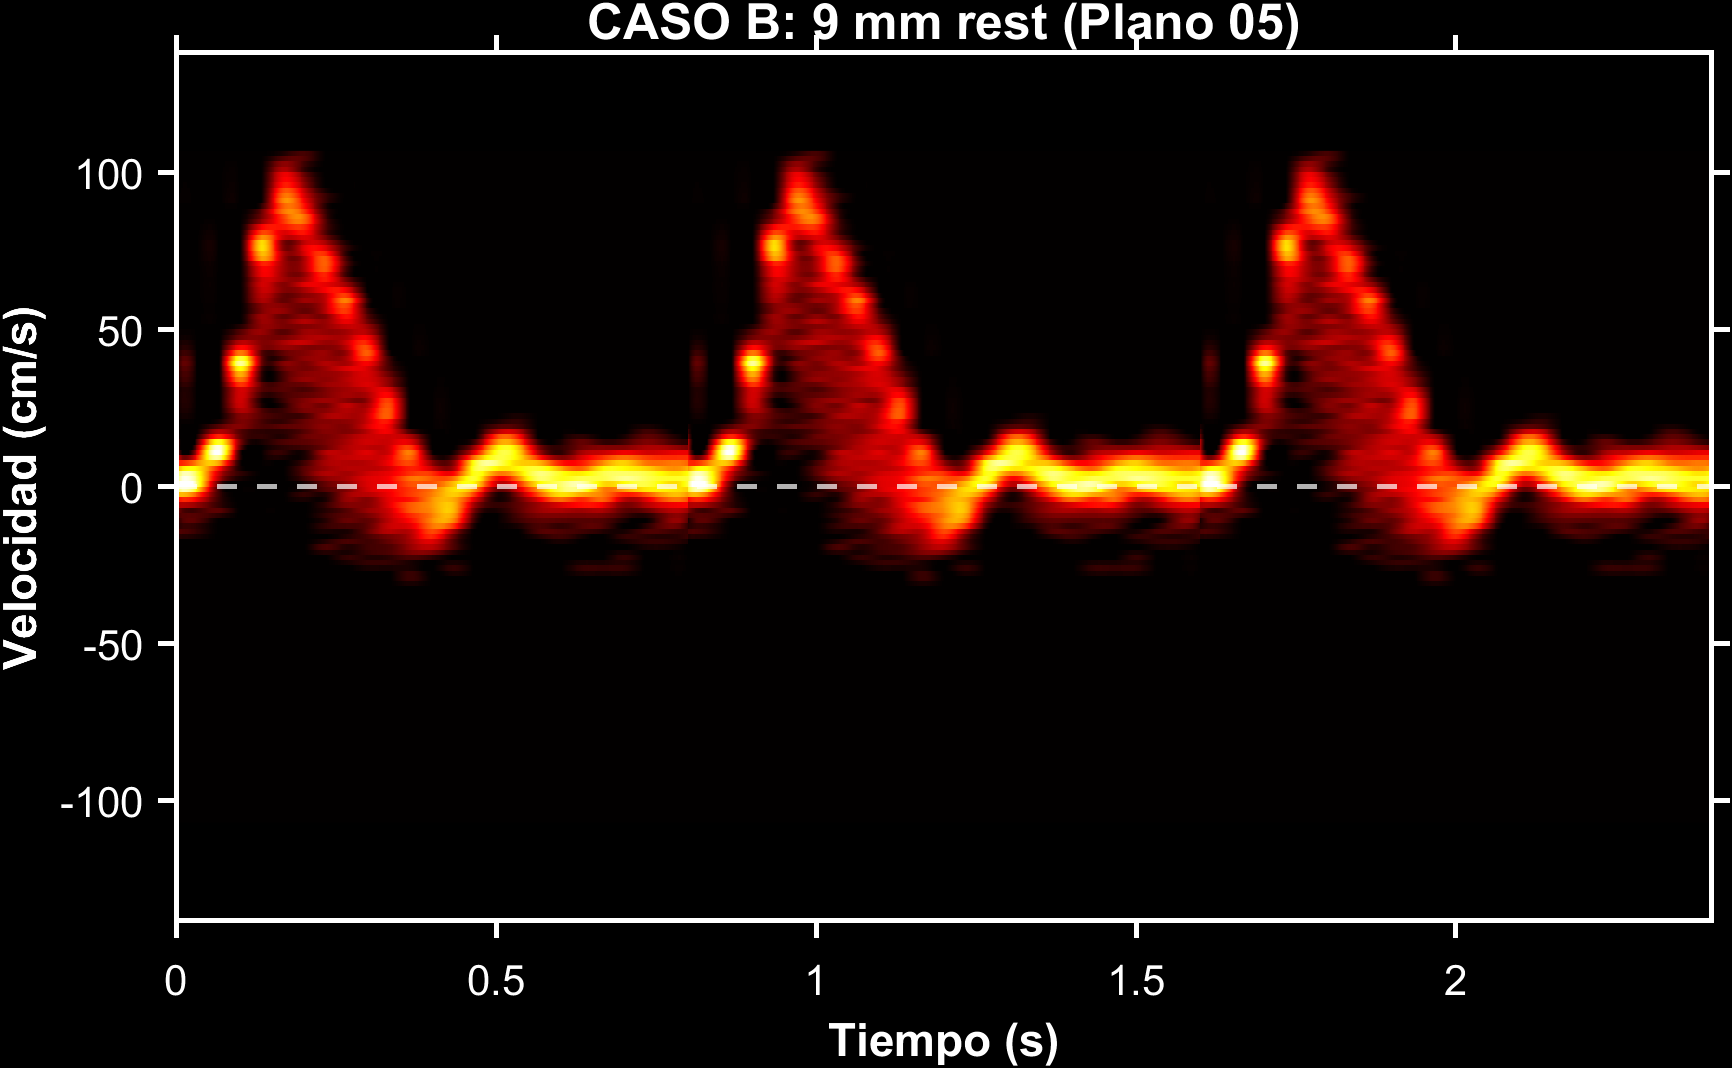
\includegraphics[width=\linewidth]{figures/anexos/9_mm_rest_Plano05.png}
            \caption{\href{https://drive.google.com/file/d/15aY5Ka3epcruwTPN9ZXKztg4-zE6n9DE/view?usp=sharing}{9 mm \textit{rest} \textbf{(Escuchar)}}}
            \label{fig:anexo_p5_9mm_rest}
        \end{subfigure}\hfill
        \begin{subfigure}{0.48\linewidth}
            \centering
            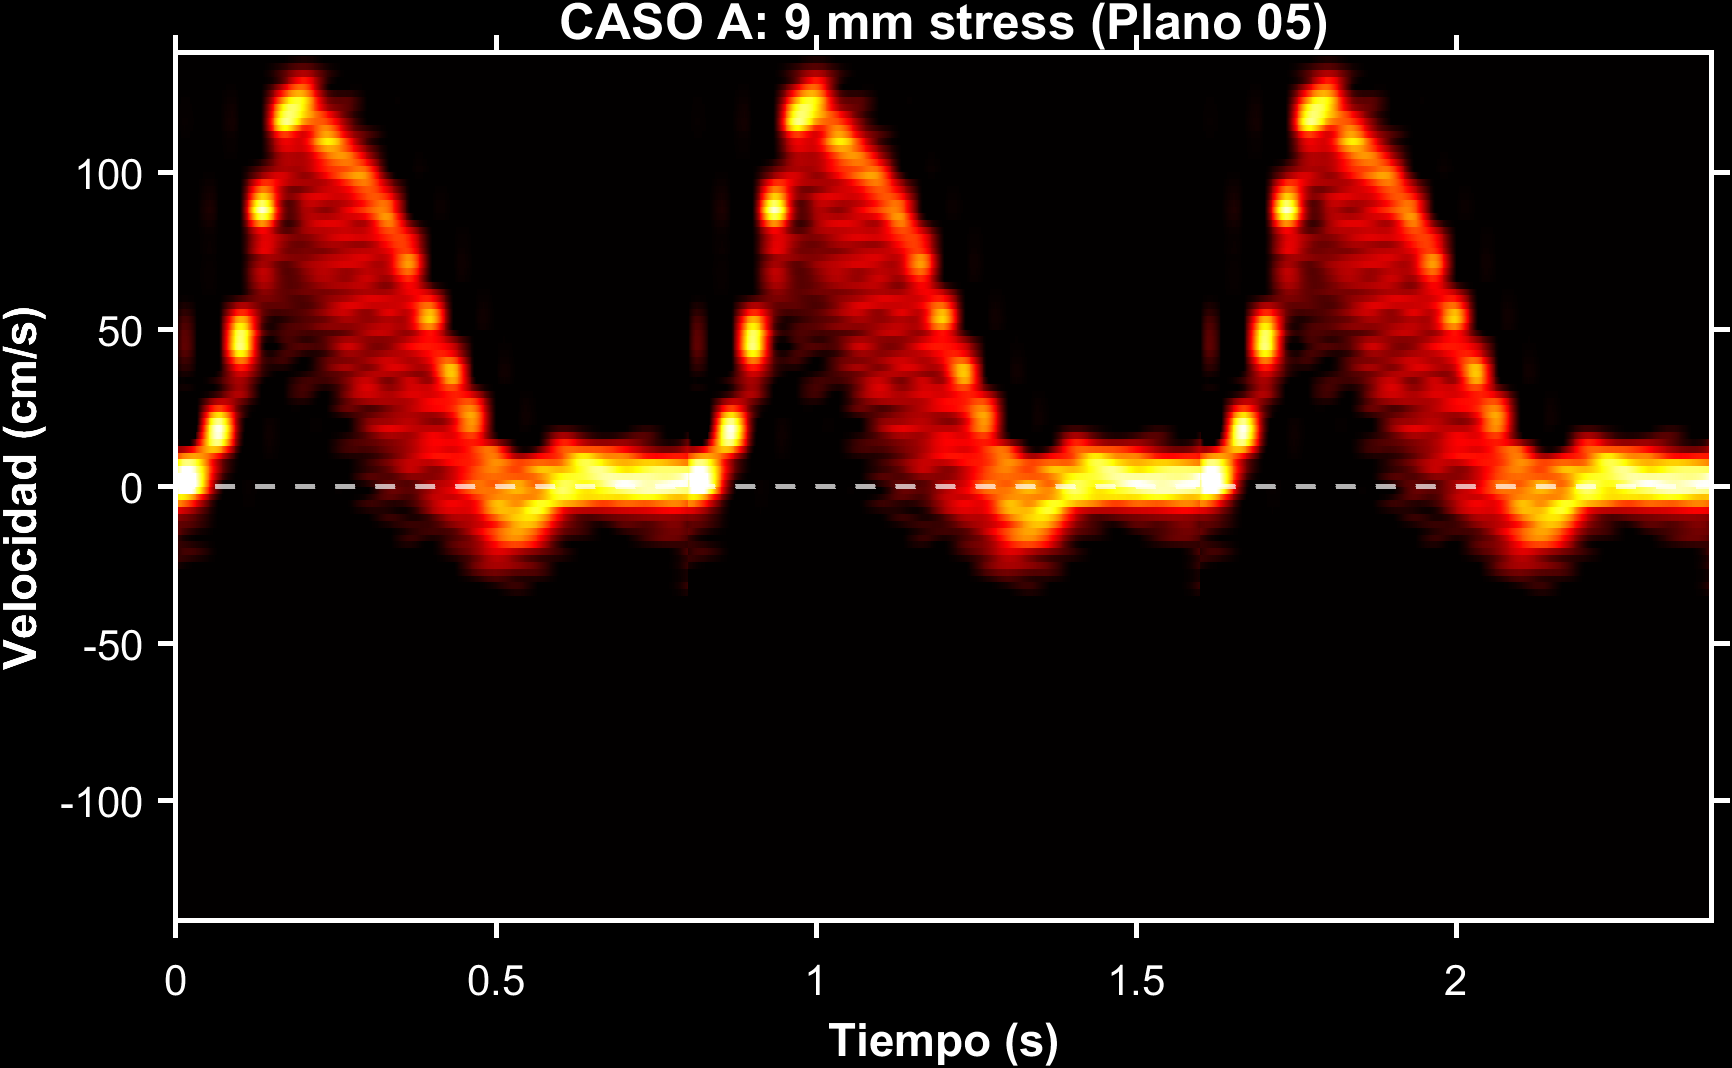
\includegraphics[width=\linewidth]{figures/anexos/9_mm_stress_Plano05.png}
            \caption{\href{https://drive.google.com/file/d/1KWstZDt0APd1gukMKM52vnXZ9ZMmdCZZ/view?usp=sharing}{9 mm \textit{stress} \textbf{(Escuchar)}}}
            \label{fig:anexo_p5_9mm_stress}
        \end{subfigure}
    \end{minipage}
    \caption{\label{fig:anexo_comparacion_p5} Comparación espectral en el plano 5 evaluando los casos Normal y 9 mm bajo condiciones de reposo y estrés. Fuente: Elaboración propia.}
\end{figure}


\subsection{Análisis comparativo extremo: Plano 85}

\begin{figure}[H]
    \centering
    \begin{minipage}{0.75\textwidth}
        \begin{subfigure}{0.48\linewidth}
            \centering
            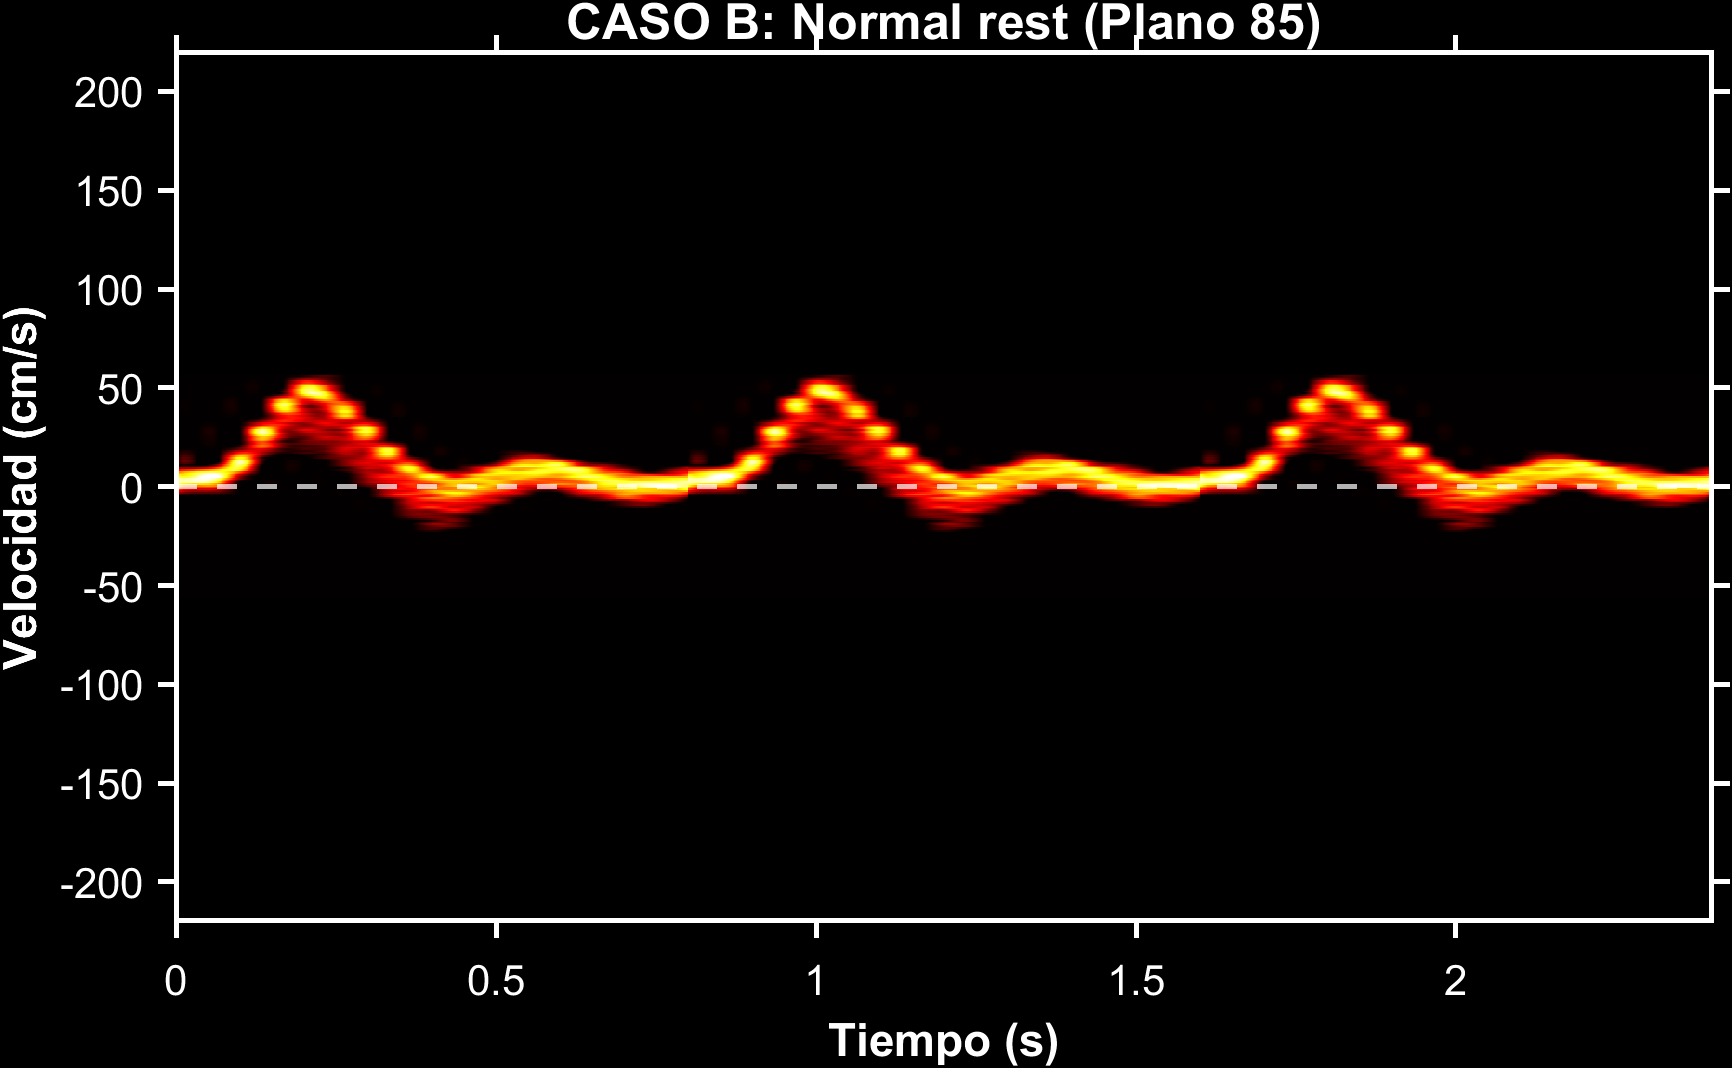
\includegraphics[width=\linewidth]{figures/anexos/Normal_rest_Plano85.png}
            \caption{\href{https://drive.google.com/file/d/1x_aCgRlC-U291iP3yWYODxnAIjABdu7s/view?usp=sharing}{Normal \textit{rest} \textbf{(Escuchar)}}}
            \label{fig:anexo_p85_normal_rest}
        \end{subfigure}\hfill
        \begin{subfigure}{0.48\linewidth}
            \centering
            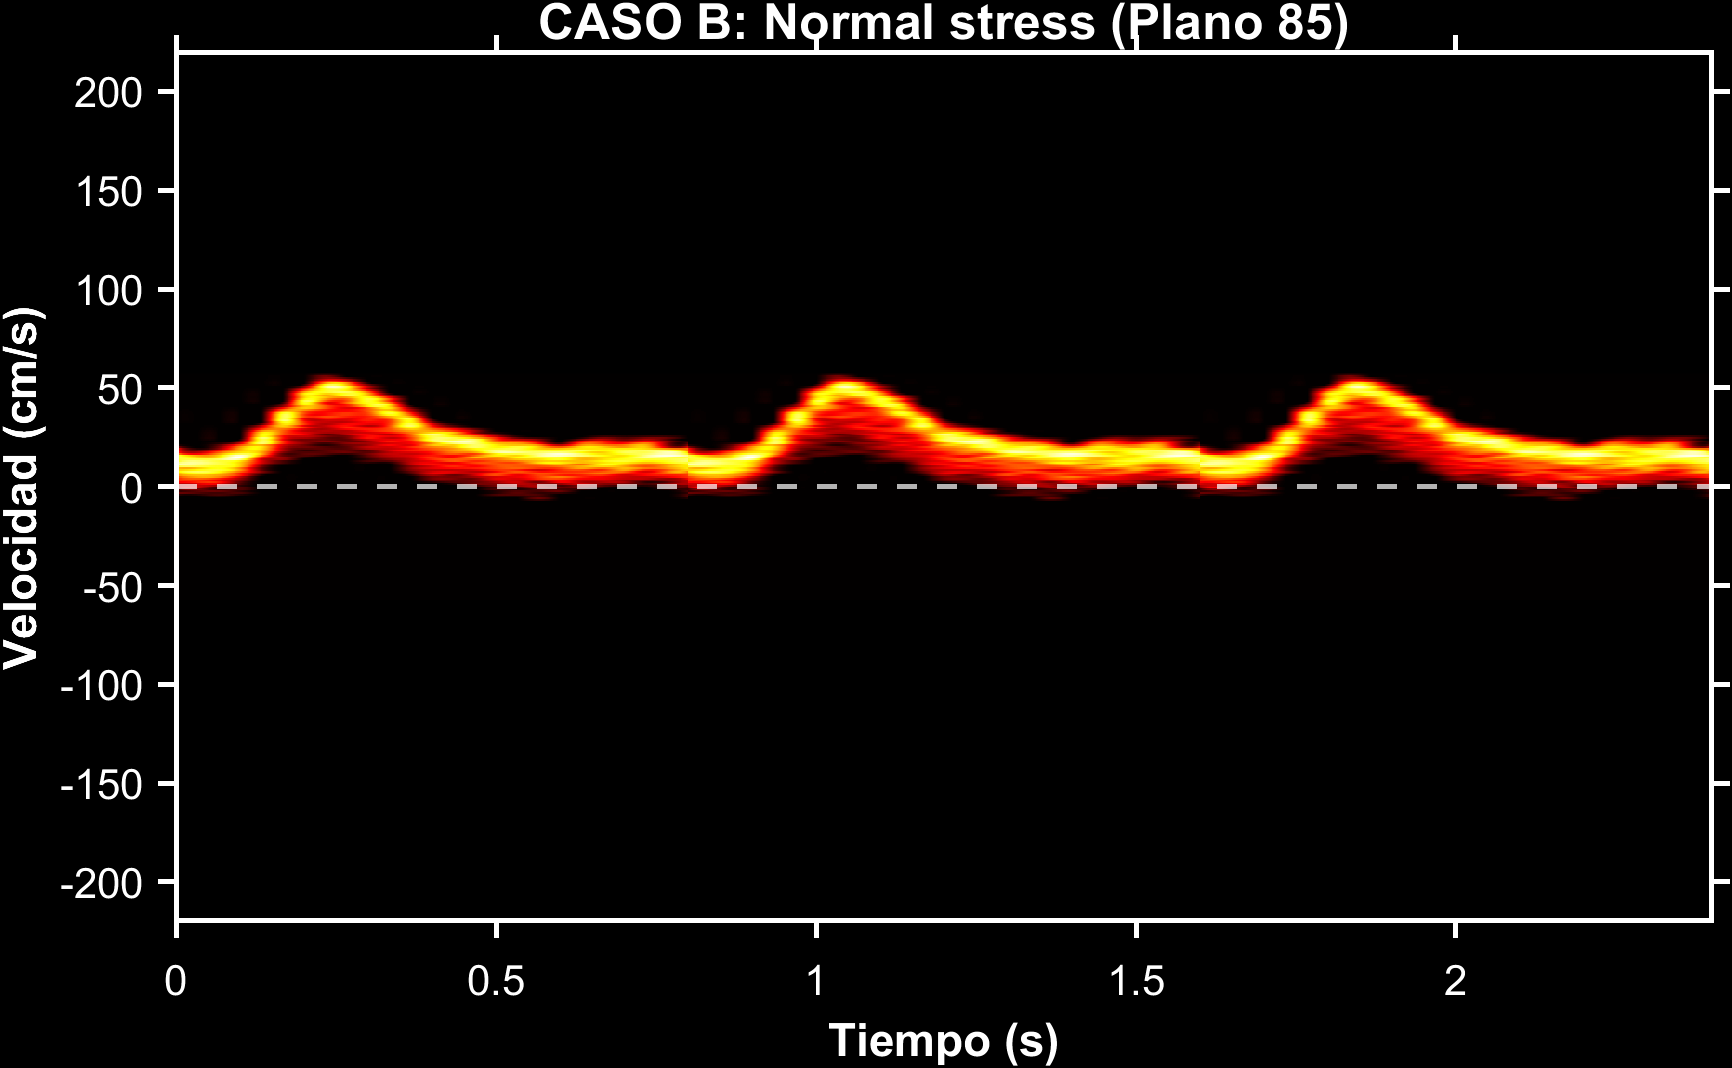
\includegraphics[width=\linewidth]{figures/anexos/Normal_stress_Plano85.png}
            \caption{\href{https://drive.google.com/file/d/1ZpgR28frecUy7BBZH10Bbx4weVoIk4Ci/view?usp=sharing}{Normal \textit{stress} \textbf{(Escuchar)}}}
            \label{fig:anexo_p85_normal_stress}
        \end{subfigure}
        
        \vspace{0.4cm}
        
        \begin{subfigure}{0.48\linewidth}
            \centering
            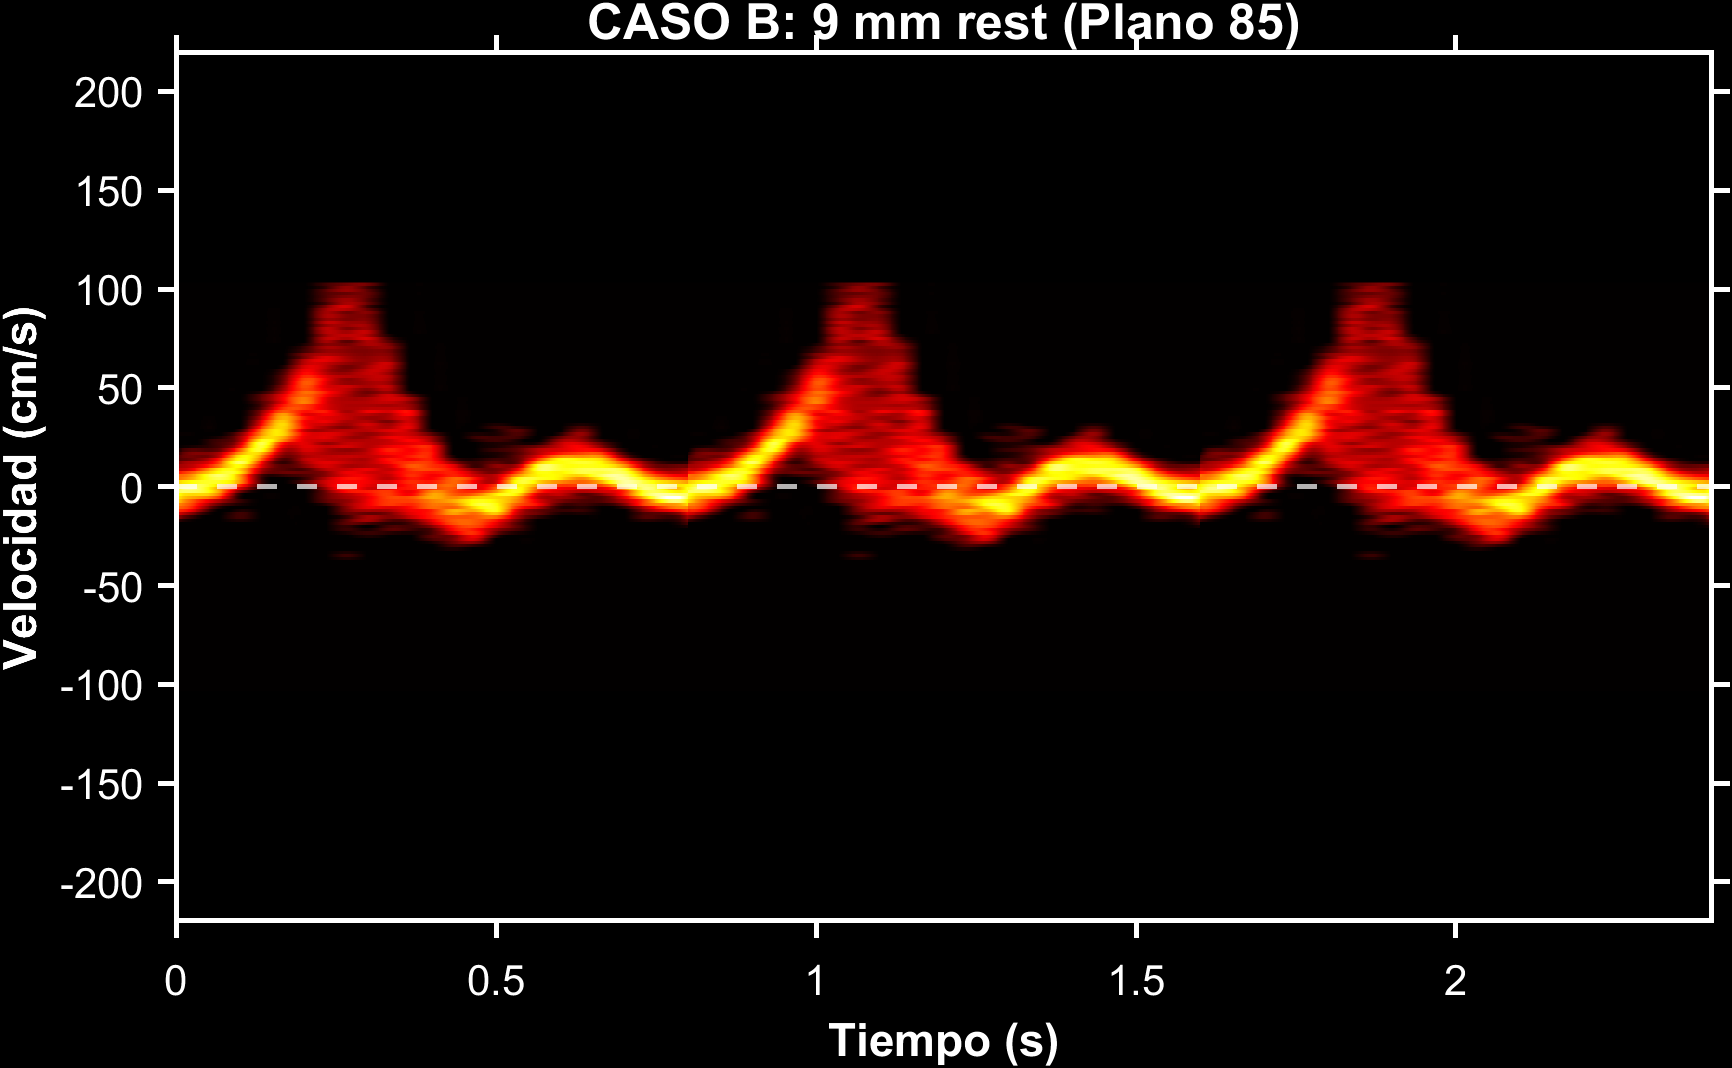
\includegraphics[width=\linewidth]{figures/anexos/9_mm_rest_Plano85.png}
            \caption{\href{https://drive.google.com/file/d/1xdobj-27zKS08QWK1PNRTL2fhcNn9-fd/view?usp=sharing}{9 mm \textit{rest} \textbf{(Escuchar)}}}
            \label{fig:anexo_p85_9mm_rest}
        \end{subfigure}\hfill
        \begin{subfigure}{0.48\linewidth}
            \centering
            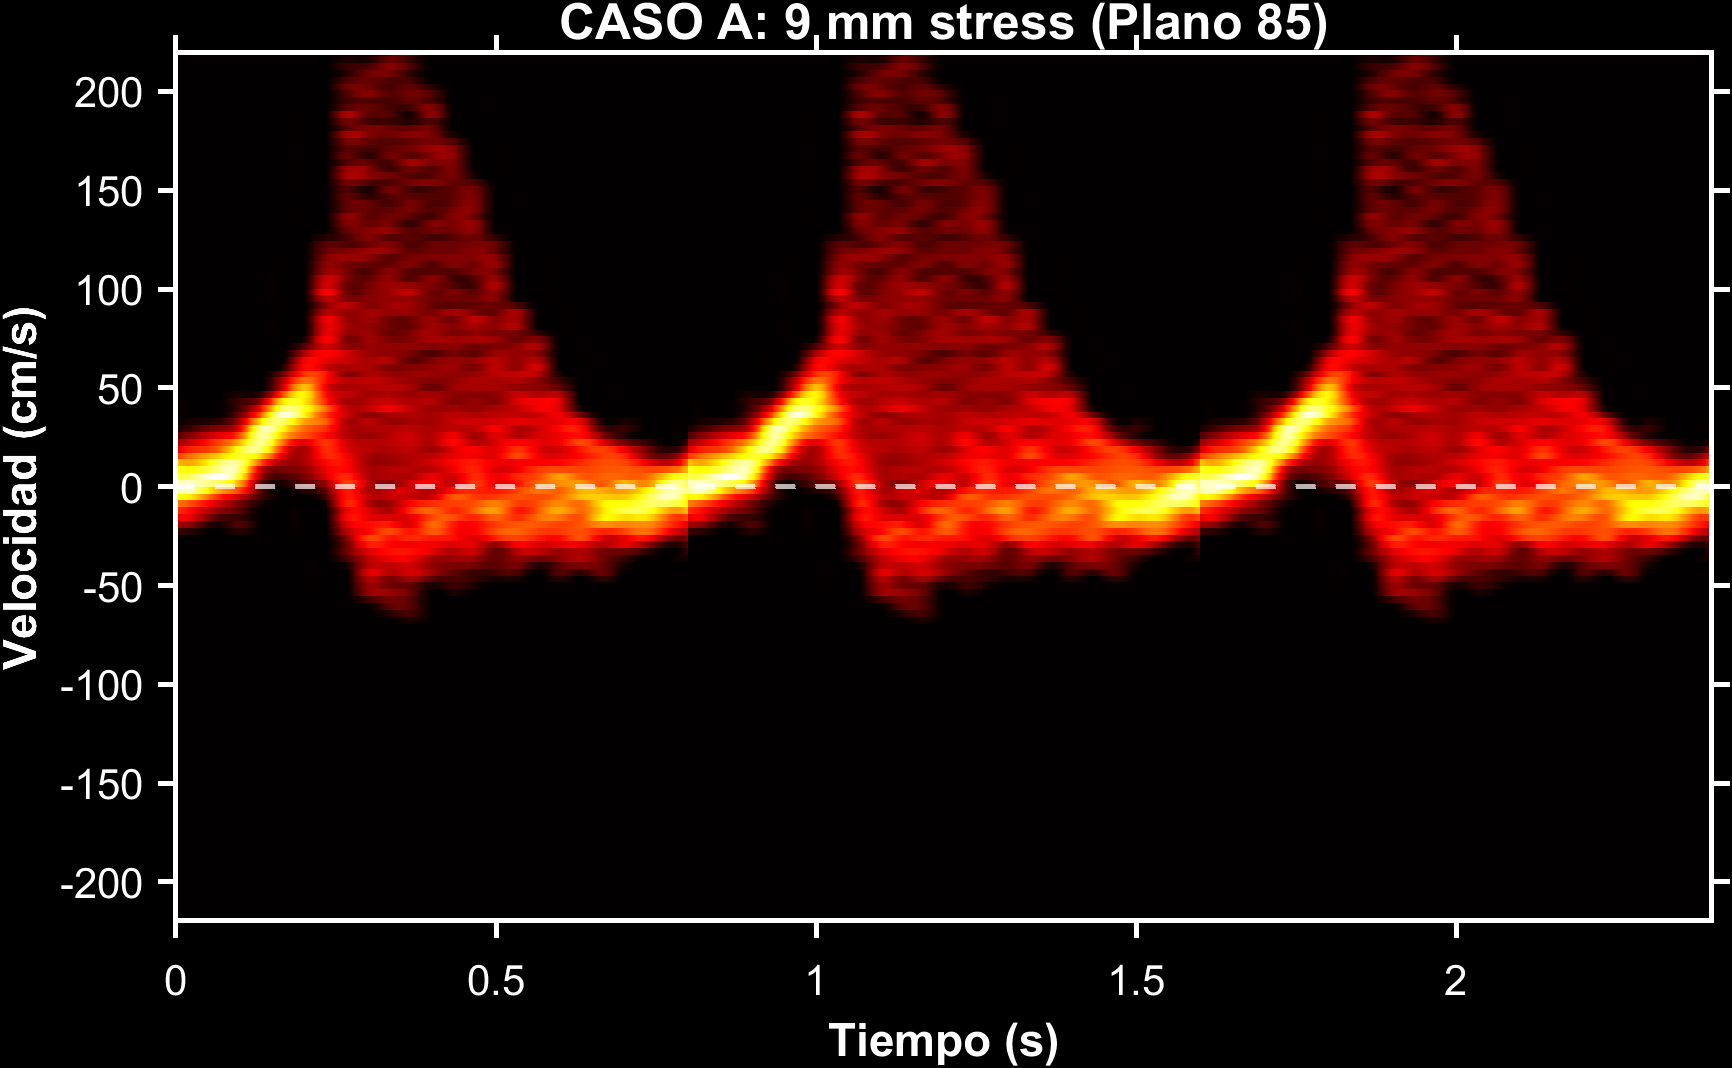
\includegraphics[width=\linewidth]{figures/anexos/9_mm_stress_Plano85.png}
            \caption{\href{https://drive.google.com/file/d/1xdobj-27zKS08QWK1PNRTL2fhcNn9-fd/view?usp=sharing}{9 mm \textit{stress} \textbf{(Escuchar)}}}
            \label{fig:anexo_p85_9mm_stress}
        \end{subfigure}
    \end{minipage}
    \caption{\label{fig:anexo_comparacion_p85} Comparación espectral en el plano 85 evaluando los casos Normal y 9 mm bajo condiciones de reposo y estrés. Fuente: Elaboración propia.}
\end{figure}